% !TeX root = ekg-mm/ekg-mm.tex
\makeatletter\def\input@path{{../../../etc/}{../../etc/}{../etc/}}\makeatother
\documentclass{whitepaper-style-doc}

\loadGlossaries

\RequirePackage{maturity-model-stuff}

%
% The following two lines make sure that chapter numbers
% start with 1 within each part.
%
\RequirePackage{chngcntr}
\counterwithin*{chapter}{part}

\loadGlossaries

%
% Title page variables
%
\title{\glsfmtshort{ekgmm}}
\def\subtitleLineA{Overview of the Maturity Model}
\def\subtitleLineB{for the \glsxtrlong{ekg}}
\author{Enterprise Knowledge Graph Foundation}
\date{\today}

\newcommand{\ekgmmContextSection} {\subsection*{\glsfmtshort{ekg} Context}}
\newcommand{\ekgmmHowEKGRequiresThisCapability} {\subsubsection*{How \glsfmtshort{ekg} requires this capability}}
\newcommand{\ekgmmHowEKGAffectsThisCapability} {\subsubsection*{How \glsfmtshort{ekg} affects this capability}}
\newcommand{\kgmmcorequestionssection}  {\subsection*{Core Questions}}
\newcommand{\kgmmscoringsection}        {\subsection*{Scoring}}

\def\ekgmmLevelOneLabel{\glsfmtshort{ekg} Initiation\,---\,Lighthouse Project}
\def\ekgmmLevelTwoLabel{Extensible Platform\,---\,reusable components}
\def\ekgmmLevelThreeLabel{Enterprise Ready\,---\,default data hub}
\def\ekgmmLevelFourLabel{Strategic Asset\,---\,operational utility}
\def\ekgmmLevelFiveLabel{Operational Ecosystem\,---\,continuous development}

\newcommand{\kgmmscoringlevelOne}  {\paragraph*{Level 1: \glsfmtshort{ekg} Initiation}}
\newcommand{\kgmmscoringlevelTwo}  {\paragraph*{Level 2: Extensible Platform}}
\newcommand{\kgmmscoringlevelThree}{\paragraph*{Level 3: Enterprise Ready}}
\newcommand{\kgmmscoringlevelFour} {\paragraph*{Level 4: Strategic Asset}}
\newcommand{\kgmmscoringlevelFive} {\paragraph*{Level 5: Operational Ecosystem}}


\typeout{ekg-mm =================================> Start Document}
\begin{document}

\typeout{ekg-mm =================================> Intro}
\part{Intro}\label{pt:ekg-mm-intro}

\bgroup

% \renewcommand{\thechapter}{\thepart.\arabic{chapter}}
% \renewcommand{\thesection}{\thechapter.\arabic{section}}
% \renewcommand{\thesubsection}{\thesection.\arabic{subsection}}
% \renewcommand{\thesubsubsection}{\thesubsection.\arabic{subsubsection}}

\chapter{Work in Progress}\label{ch:ekg-mm-work-in-progress}

\improve[inline]{%
    On the first page we should have caveats about this being a work in progress and encourage people to get involved,
    whether a member or not, including just providing feedback. Link to the sign up page on the website
}

\chapter{Executive Summary}\label{ch:ekg-mm-executive-summary}

The \gls{ekgmm} is the industry-standard definition of the capabilities required for an \gls{ekg} and
of the generic capabilities in any given organization that are affected by \gls{ekg}.

It establishes standard criteria for measuring progress and sets out the practical questions that all involved
stakeholders ask to ensure trust, confidence and usage flexibility of data.
Each capability area provides a business summary denoting its importance, a definition of the added value from
semantic standards and scoring criteria based on five levels of defined maturity.

The \gls{ekgmm} is a capability model designed to promulgate best practices across the knowledge graph community.
It covers essential capabilities as well as standard evaluation criteria required for the design, implementation,
and maintenance of an \gls{ekg}.

The initial model was developed by \agnos and is being managed as an open-source initiative by the \gls{ekgf}.

%
% Adding the "strategic objectives" chapter in draft mode
%
\ifoptionfinal{}{
    \chapter{Strategic Objectives}
%
% TODO: Add all the concepts to the index
%
\begin{itemize}[leftmargin=2in,font=\bfseries]
  \item [Business Strategy] corporate objectives, use cases and organizational mechanisms necessary for sustainable business value from the \glsxtrfull{ekg}
  \begin{itemize}[labelwidth=1.5in,leftmargin=0in]
    \item [Corporate Goals] Alignment (shared vision) on why the organization is building a knowledge graph
    \item [Business Unit Goals] Support of the \glsfmtshort{ekg} value proposition\index{\glsfmtshort{ekg}!value proposition} by
          key \glsxtrshort{lob} \iindex{stakeholders}
    \item [Organizational Considerations] Operational and resource plans for \gls{ekg} strategy implementation and governance
  \end{itemize}
  \item [Data Strategy] enterprise data management framework (policies, target data architecture, quality assurance,
        governance) necessary to support the knowledge graph environment
    \begin{itemize}[labelwidth=1.5in,leftmargin=0in]
      \item [Data Goals \& Objectives] Importance of unique identification and the value of unambiguous shared meaning
      \item [Knowledge Graph Positioning] Role of the \glsxtrshort{ekg} as the underlying \iindex{data!fabric}
            for the organization
      \item [Business Case] \gls{roi} of linked data as an essential component of operational infrastructure
    \end{itemize}
  \item [Technology Strategy] environment for successful knowledge graph implementation including direction for
        \iindex{physical infrastructure}, applications and \iindex{process automation}
    \begin{itemize}[labelwidth=1.5in,leftmargin=0in]
      \item [Infrastructure Strategy] Physical infrastructure (i.e. \iindex{cloud}, \iindex{containerization},
            software layer) for the \glsxtrshort{ekg}
      \item [Application Strategy] Applications approach including rationalization, build vs. buy and standards adoption
      \item [Automation Strategy] Use of \glsfirst{ai} and \iindex{robotic process automation}
    \end{itemize}
\end{itemize}

~\\

\begin{description}[nosep,font=\bfseries]

  \item [High-Level Business Goals]
  Create integrated views, enhance product innovation, profile behavior, 
  determine preferences, understand relationships, implement target selling, 
  determine customer and product \gls{roi}, perform predictive modeling,
  define social connections, segment customers, enhance product satisfaction, 
  understand the dynamics of the market, operate with more agility, 
  maximize time-to-market.
  ~\\
  \begin{itemize}
    \item Do LOB stakeholders clearly understand the relationship between data management and business objectives
    \item Is all the data that is important to meet business priorities been defined and classified
    \item Is the data management strategy aligned with business priorities, implementation plans, technical capabilities and operational processes
    \item Has the data management strategy been mapped to business and organizational objectives
    \item Have business use cases and user stories been defined and aligned to data concepts
    \item Have LOB business outcomes (and dependencies) been defined and sequenced across the organizations
    \item Is there alignment between organizational/business objectives and data (concepts and repositories)
    \item Has the organization defined and aligned data metrics and KPIs with business objectives
    \item Has the organization defined the business architecture for both strategic and tactical objectives
    \item Is the data strategy aligned with lines of business objectives
    \item Have service level agreements been defined and verified for critical systems and processes
    \item Are the lines of business engaged in (and understand the rationale of) the data management program
    \item Are lines of business and functional organizations committed and accountable to the data management objectives
  \end{itemize}

  ~\\

  \item [High-Level Technology Goals]
  Optimize infrastructure investments, automate business processes, 
  perform security surveillance, protect privacy, support continuous deployment. \\

  \begin{itemize}
    \item Does an integrated technology architecture strategy exist (and has it been implemented)
    \item Have IT and platform governance processes been defined and aligned with the data management strategy
    \item Do executive stakeholders have confidence in the ability of IT to manage realignment of fragmented architecture to meet strategic objectives (i.e. customer 360 and automated regulatory reporting)
    \item Has the data storage strategy been defined and aligned with the goals of data reconstruction, security and archive
  \end{itemize}

  ~\\

  \item [High-Level Data Goals]
  Adopt data management principles of identity and meaning, 
  monitor and ensure F-F-P quality, ensure data accessibility, 
  eliminate data duplication, reduce reconciliation, 
  govern the data lifecycle, control data at source, 
  control the data manufacturing process. \\

  \begin{itemize}
    \item Is there a clearly defined and sanctioned data strategy for the organization (aligned to organizational and business objectives)
    \item Does the organization have “data management delusions” and are they aware of their fallacy
    \item Does the organization have a plan on how to execute their data-centric strategy
    \item Has the data management business case been linked to organizational strategy and business pain points
    \item Are data requirements defined and aligned with funding processes
    \item Is there a mechanism for obtaining and verifying data management feedback from stakeholders
    \item Have the full suite of policies for data management been defined, approved and implemented
    \item Does the organization document and track the data production and consumption process
          (where data lives, the applications that are used, how it flows and where transformation occurs)
    \item Have logical and conceptual data models been defined and verified
    \item Is meaning of data in \glspl{sor} verified and locked down
    \item Are the criteria for designating criticality (and other classifications) consistent and scalable
    \item Does the organization have a data management and governance strategy to deliver against business objectives
    \item How does the organization evaluate the costs and effectiveness of the data strategy
    \item Has the data management strategy been translated into a operational roadmap
    \item Is funding and resource allocation plan in place to deliver against the data strategy
    \item Are communications, positioning and training programs about data management designed and operational
  \end{itemize}

  ~\\

  \item [High-level Organizational Goals]
  Perform flexible analysis, trust, operational resiliency, achieve efficiency/\-save money,
  comply with regulatory obligations, comply with contractual obligations, avoid fines,
  mitigate risk, preventing fraud, manage organizational change, enhance worker satisfaction,
  aggregate reporting, negotiate smart contracts with vendors, leverage capital,
  enhance market position, manage TCO and profitability. \\

  \begin{itemize}
    \item Does the organization view data as an instrument to transform the business
    \item Do the executive stakeholders within the organization understand the reasons why data is not harmonized across repositories and business processes (causes of incongruence)
    \item Do executive stakeholders understand the business rationale for establishing a “data control environment”
    \item Have high-level organizational goals been translated into data concepts
    \item Are knowledge workers focused on value-added activities
    \item Are key stakeholders committed to the principles and priorities of the data management program
    \item Does the organization have the skill sets and people talent to implement the data management strategy
  \end{itemize}

\end{description}











}
\chapter{Structure}\label{ch:ekg-mm-structure}

The \glsfirst{ekgmm} is a collection of capabilities structured in a relatively simple 4x5 matrix of
\textit{capability domains} and \textit{maturity levels}.

\begin{figure}[ht]
    \centering
    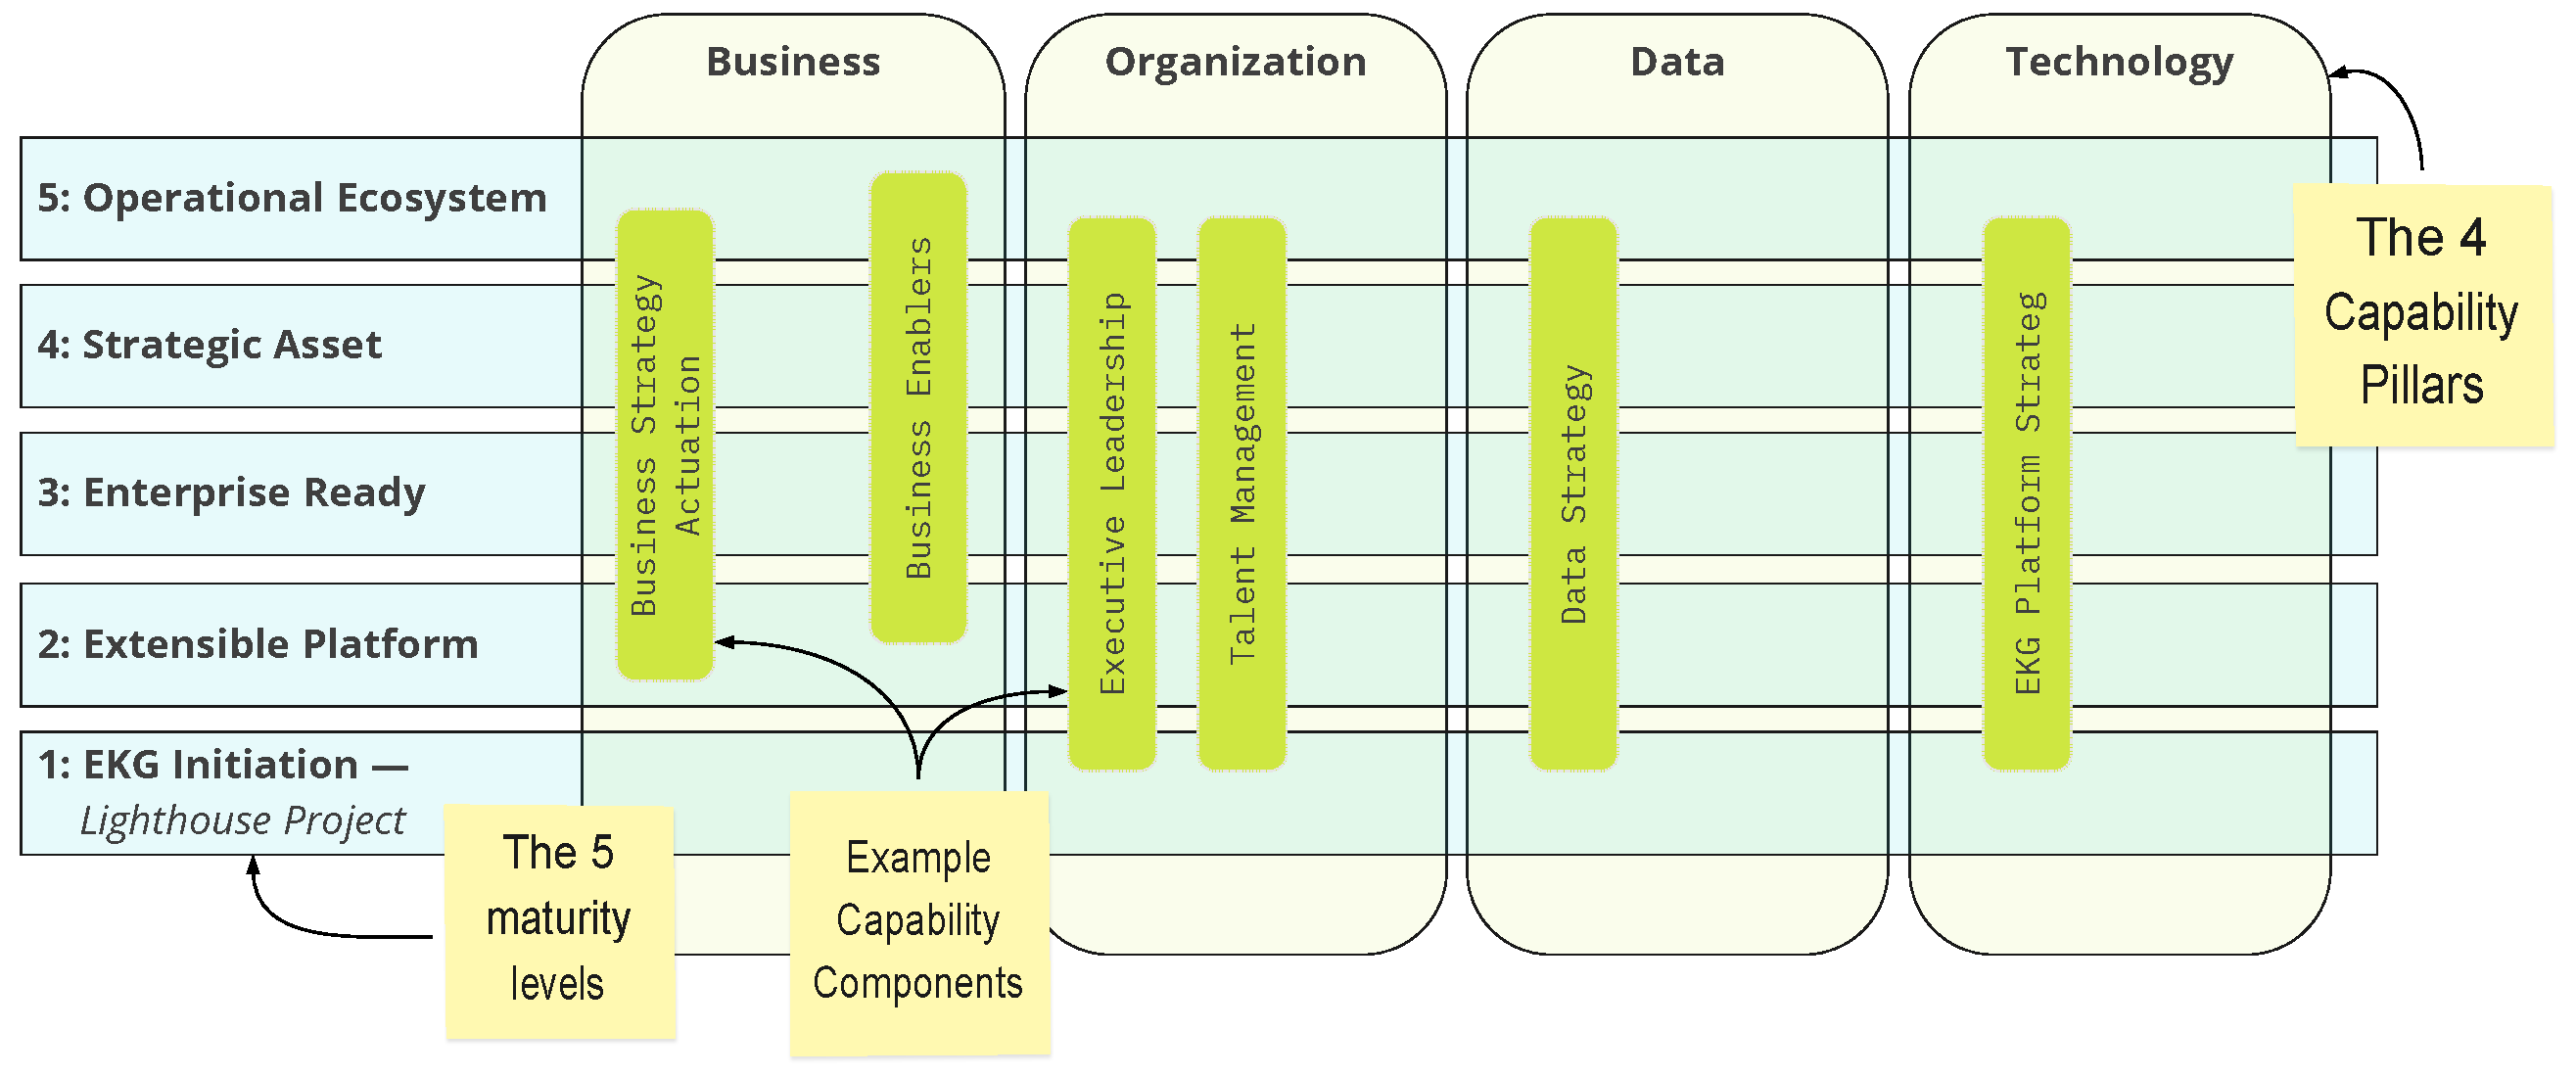
\includegraphics[width=\textwidth]{../images/ekg-mm-structure.pdf}
    \caption{\glsfmtshort{ekgmm} Structure}
    \label{fig:ekg-mm-structure}
\end{figure}

\section{The Four Capability Pillars}\label{sec:ekg-mm-the-four-pillars}
\input{../../ekg-mm/fragments/ekg-mm-capability-domains-summary.tex}

\subsection{Business Pillar}\label{subsec:ekg-mm-the-four-pillars-business-pillar}

All Business-side capabilities including~\nameref{ch:ekg-mm-business-strategy-actuation},
\index{business!strategy}~\nameref{ch:ekg-mm-business-model-elaboration},
\index{business!architecture!elaboration}~\nameref{ch:ekg-mm-business-enablers}, Alignment,
\nameref{sec:ekg-mm-business-operating-model} and others.
Does not include all the actual Business Capabilities\index{business!capabilities} that
an enterprise may have themselves.

Addresses the \iindex{audience} of personas on the business-side of an enterprise, C-level,
\gls{lob} execs,\index{executive}\index{persona!executive}
corporate planners,\index{corporate planner}\index{persona!corporate planner}
business architects\index{business!architects}, product owners\index{product owner}\index{persona!product owner},
management consultants\index{management consultant}\index{persona!management consultant} and so forth.

\subsection{Organization Pillar}\label{subsec:ekg-mm-the-four-pillars-organization-pillar}

All relevant Organizational Capabilities including~\nameref{ch:ekg-mm-executive-leadership},
~\nameref{ch:ekg-mm-product-ownership},
~\nameref{ch:ekg-mm-delivery-management},
~\nameref{ch:ekg-mm-organizational-culture}, and
~\nameref{ch:ekg-mm-organizational-capabilities}.

Addresses the \iindex{audience} of people that are neither business, data nor tech such as financial execs and experts, risk
execs and experts, program/portfolio/project managers, HR execs and experts and so forth.

\subsection{Data Pillar}\label{subsec:ekg-mm-the-four-pillars-data-pillar}

All Data (Management) capabilities including~\nameref{ch:ekg-mm-data-strategy}.
\index{strategy!data strategy}

Addresses the \iindex{audience} of people in the data-management and data-governance departments.

\subsection{Technology Pillar}\label{subsec:ekg-mm-the-four-pillars-technology-pillar}

All Technology Capabilities including~\nameref{ch:ekg-mm-technology-strategy},
~\nameref{ch:ekg-mm-technology-execution}, and
~\nameref{ch:ekg-mm-user-interface}.
\index{strategy!technology strategy}

Addresses the \iindex{audience} of technologists, technical architects, developers, infrastructure execs and experts,
security execs and experts etc.



\section{The five maturity levels}\label{sec:the-five-maturity-levels}

This document will refer\,---\,for each capability\,---\,to the five maturity levels.

\subsection{Level 1: \ekgmmLevelOneLabel}

The domain of internal \glspl{poc}, pilots or\,---\,ideally\,---\,"\glspl{lighthouse-project}".
The focus is usually on specific targeted baseline use cases constructed using isolated ontologies.
The champions are visionaries who have assembled a specialist team for implementation\,---\,possibly the
start of the \glsfirst{ekg:coe}.
Funding is likely to be project-based and designed to demonstrate capabilities.

\begin{itemize}[leftmargin=1in,font=\bfseries]

    \item[Business]     Stakeholders recognize business opportunities in scaling and amplifying capabilities
                        through \glspl{ekg}.
                        The first internal champion is seeking to socialize strategic business cases,
                        supports innovation, and is willing to take on the disruption challenge.
    \item[Data]         Core data management capabilities (\gls{operating-model}, inventory, data architecture,
                        \hyperref[sec:ekg-mm-vocabularies]{vocabularies, business glossary or terminology},
                        pipeline management, etc.) are being performed.
                        Specific use cases are being implemented with specialist teams for the pilot initiative.
    \item[Technology]   Technology strategy is focused on experimentation and innovation.
                        Manual data transformation and targeted ETL is underway for the pilot.
                        Limited infrastructure and dedicated efforts to build initial knowledge graph components.
    \item[Organization] Champions are internal visionaries who have assembled a specialist team for implementation.
                        The pilot is sanctioned and funded.
                        Knowledge acceleration is being addressed.
                        Overall organizational support is emerging
\end{itemize}

\subsection{Level 2: \ekgmmLevelTwoLabel}

The domain of parallel knowledge graph activities, implementing multiple (related) use cases on the same platform.
The organization is creating reusable architecture\,---\,i.e. "the \gls{ekg:platform}"\,---\,based
on \citefield{ekgprinciples}{title}.
The \glsfirst{ekg:coe} is created.
Funding is likely to be at the \gls{lob} level and starts to (partly) come from \gls{bau} budgets.

\begin{itemize}[leftmargin=1in,font=\bfseries]

    \item[Business]     Stakeholders adopt a “knowledge-centric” mindset in their tactics to strengthen focus on
                        strategic business value.
                        Management elevates the knowledge graph as an organizational and funding priority.
    \item[Data]         Critical data elements are prioritized in the ontology.
                        Approach to identity and meaning resolution is established.
                        Use case trees are defined and modeled to capture shared data relationships.
                        The knowledge graph is becoming the central point for integration.
    \item[Technology]   Reusable architecture based on \citefield{ekgprinciples}{title}.
                        Core software development design approaches are being established and incorporated
                        into strategy.
                        CTO focuses on extending pilot initiatives for additional leverage.
    \item[Organization] \Gls{operating-model} of collaboration is implemented to support the knowledge graph.
                        The Center of Excellence and DataOps environment is initiated.
                        Budget and implementation strategy are based on agile and synchronized with the
                        use case tree methodology.
\end{itemize}

\subsection{Level 3: \ekgmmLevelThreeLabel}

The establishment of a secure, scalable and resilient \gls{ekg:platform} for business-critical strategic use cases.
Resources for the design and build of operational systems are defined and coordinated.
The knowledge graph is now really an \myuline{Enterprise} Knowledge Graph (EKG) that serves as the
semantic data fabric\index{data fabric} for the organization.
Ownership, governance, and funding are managed at the enterprise level and coordinated by the \gls{ekg:coe} that
oversees the full life-cycle of use cases from inception to deployment and beyond.
Long-term "operate \& optimize" processes are in place.

\begin{itemize}[leftmargin=1in,font=\bfseries]

    \item[Business]     Strong collaboration between various business and support units to prioritize
                        strategic business cases.
    \item[Data]         Inventory is embedded into the \gls{ekg} and linked to governance.
                        Data is expressed as formal ontologies, onboarded into the \gls{ekg} and searchable.
                        Data flows are defined and modeled.
                        The \gls{ekg} is the authoritative source for data.
    \item[Technology]   Commitment to the \gls{ekg} as the strategic infrastructure for the organization.
                        IaC and continuous deployment adopted and implemented.
                        Cloud architecture defined for elasticity.
                        Datapoint security and authentication processes implemented
    \item[Organization] The \gls{ekg} is recognized as a core service for the enterprise.
                        Enterprise-wide ownership and funding processes are operational.
                        The \gls{ekg:coe} is a stand-alone \gls{bau} department.
\end{itemize}

\subsection{Level 4: \ekgmmLevelFourLabel}

The \gls{ekg} is understood as strategic infrastructure\,---\,as an operational utility\,---\,for the organization
and the authoritative source for most data (except for data that originates from core legacy systems).
It supports structural application rationalization\index{rationalization}, high-level and high-quality \gls{ai}
that can take over many tasks from humans and process automation.
Strategic funding is based on the vision of executive management and fully embraced by the Board of Directors.
All core data management capabilities have been achieved.

\subsection{Level 5: \ekgmmLevelFiveLabel}

The \gls{ekg} is central to systems and business processes.
It has been fully integrated into both internal operations and external supply chain partners.
Workflows and approval steps are fully automated.
Entitlements and access rights are controlled by the \gls{ekg}.
Inference and reasoning capabilities are used for advanced \gls{ai} use cases.

\section{Capability Template}

The general layout, in this document, of each capability looks as follows:

\subsection*{Capability}

[The title of the capability]

\subsubsection*{Description}

[Tagline, a short one sentence description of the Capability]

[Description of the capability]

\subsubsection*{Contribution to \glsfmtshort{ekg}}

[How the capability as part of the EKG contributes to the enterprise]

[Including traceability to EKG Principles where relevant]

\subsubsection*{Contribution to the Enterprise}

[How the capability as part of the EKG contributes to the enterprise]

\subsubsection*{Dimensions}

[General dimensions/questions being measured by the criteria at different Levels]

[The following are candidate general questions]

\begin{itemize}
    \item Level of required skills available (e.g. trained people)
    \item Level of resources available (e.g. infrastructure, tools)
    \item Level of defined processes available
    \item Scope of applicability
    \item Questions specific to the capability
\end{itemize}

\subsubsection*{Levels 1 \textendash 5}

[Description of level]

[Criteria, drawing on the Dimensions]


\todo[inline]{Explain difference between "capability" and "use case"}

\todo[inline]{Explain why certain capabilities are mentioned in this document and why others are not}

\todo[inline]{How to use the model?}

\todo[inline]{Can be used for?}

\todo[inline]{Benchmarking industry}




\pagebreak
\chapter{Overview}\label{ch:ekg-mm-overview}

Without showing the levels of the maturity model, here is an overview of the taxonomy of pillars, components,
capabilities, and the measurable abilities or summaries.

%
% Most of the rest of this file has been copied & pasted from the Excel spreadsheet
% that MIA is maintaining, via the Tables Generator website 
% at https://www.tablesgenerator.com/latex_tables#
%
% So there is no need to manually maintain this file, unless we decide to make
% everything in this table a link and give up the spreadsheet.
%
% The following changes have been made to the generated output:
%
% 1. Remove "\color[HTML]{FFF} " which causes issues. 
% 2. Insert the line \scriptsize just after \begin{table}[]
% 3. In the first column, change text like "\textbf{A. Business}" into
%    "\rotatebox{90}{\textbf{A. Business}}"
%
\bgroup

\newcommand{\setComponentColor}[1]{
    \colorlet{componentColor}{#1}
}
\newcommand{\componentLabel}[2]{
    \cellcolor{#1}\textbf{\ref{#2}~\nameref{#2}}
}
\newcommand{\labelCB}[2]{\multirow{-#1}{*}{\componentLabel{componentBusinessColor}{ch:ekg-mm-a-#2}}}
\newcommand{\labelCD}[2]{\multirow{-#1}{*}{\componentLabel{componentDataColor}{ch:ekg-mm-b-#2}}}
\newcommand{\labelCT}[2]{\multirow{-#1}{*}{\componentLabel{componentTechnologyColor}{ch:ekg-mm-c-#2}}}
\newcommand{\labelCO}[2]{\multirow{-#1}{*}{\componentLabel{componentOrganizationColor}{ch:ekg-mm-d-#2}}}


\newcommand{\setPillarColor}[1]{
    \def\pillarColor{#1}
}
\newcommand{\pillarLabel}[2]{
    \cellcolor{#1}{\rotatebox{90}{\textbf{\ref{#2}~\nameref{#2}}}}
}
\newcommand{\labelPB}[2]{\multirow{-#1}{*}{\pillarLabel{pillarBusinessColor}{pt:ekgmm-#2}}}
\newcommand{\labelPD}[2]{\multirow{-#1}{*}{\pillarLabel{pillarDataColor}{pt:ekgmm-#2}}}
\newcommand{\labelPT}[2]{\multirow{-#1}{*}{\pillarLabel{pillarTechnologyColor}{pt:ekgmm-#2}}}
\newcommand{\labelPO}[2]{\multirow{-#1}{*}{\pillarLabel{pillarOrganizationColor}{pt:ekgmm-#2}}}


\def\cellPA{\cellcolor{pillarBusinessColor}}
\def\cellPB{\cellcolor{pillarDataColor}}
\def\cellPC{\cellcolor{pillarTechnologyColor}}
\def\cellPD{\cellcolor{pillarOrganizationColor}}

\def\cellCA{\cellcolor{componentBusinessColor}}
\def\cellCB{\cellcolor{componentDataColor}}
\def\cellCC{\cellcolor{componentTechnologyColor}}
\def\cellCD{\cellcolor{componentOrganizationColor}}

\def\cellKA{\cellcolor{capabilityBusinessColor}}
\def\cellKB{\cellcolor{capabilityDataColor}}
\def\cellKC{\cellcolor{capabilityTechnologyColor}}
\def\cellKD{\cellcolor{capabilityOrganizationColor}}

\def\cellMA{\cellcolor{measurementBusinessColor}}
\def\cellMB{\cellcolor{measurementDataColor}}
\def\cellMC{\cellcolor{measurementTechnologyColor}}
\def\cellMD{\cellcolor{measurementOrganizationColor}}

\newcommand{\labelKA}[1]{\cellKA \ref{sec:ekg-mm-a-#1} & \cellKA \nameref{sec:ekg-mm-a-#1}}
\newcommand{\labelKB}[1]{\cellKB \ref{sec:ekg-mm-b-#1} & \cellKB \nameref{sec:ekg-mm-b-#1}}
\newcommand{\labelKC}[1]{\cellKC \ref{sec:ekg-mm-c-#1} & \cellKC \nameref{sec:ekg-mm-c-#1}}
\newcommand{\labelKD}[1]{\cellKD \ref{sec:ekg-mm-d-#1} & \cellKD \nameref{sec:ekg-mm-d-#1}}

\newcommand{\taglineA}[1]{\cellMA \input{../../ekg-mm/fragments-capability-tagline/a-#1}}
\newcommand{\taglineB}[1]{\cellMB \input{../../ekg-mm/fragments-capability-tagline/b-#1}}
\newcommand{\taglineC}[1]{\cellMC \input{../../ekg-mm/fragments-capability-tagline/c-#1}}
\newcommand{\taglineD}[1]{\cellMD \input{../../ekg-mm/fragments-capability-tagline/d-#1}}

\begin{table}[ht]
    \centering\fontsize{7pt}{8pt}\selectfont
    \setlength\tabcolsep{2pt}
    \begin{tabular}{@{}cclcl@{}}
    \textbf{Pillar} & \textbf{Component} & & \textbf{Capability} & \textbf{Measurable ability}                                              \\
    \cellPA         & \cellCA            & \labelKA{1-1} & \taglineA{1-1} \\
    \cellPA         & \cellCA            & \labelKA{1-2} & \taglineA{1-2} \\
    \cellPA         & \labelCB{3}{1}     & \labelKA{1-3} & \taglineA{1-3} \\
    \cellPA         & \cellCA            & \labelKA{2-1} & \taglineA{2-1} \\
    \cellPA         & \cellCA            & \labelKA{2-2} & \taglineA{2-2} \\
    \cellPA         & \labelCB{3}{2}     & \labelKA{2-3} & \taglineA{2-3} \\
    \cellPA         & \cellCA            & \labelKA{3-1} & \taglineA{3-1} \\
    \cellPA         & \cellCA            & \labelKA{3-2} & \taglineA{3-2} \\
    \cellPA         & \cellCA            & \labelKA{3-3} & \taglineA{3-3} \\
    \labelPB{10}{a} & \labelCB{4}{3}     & \labelKA{3-4} & \taglineA{3-4} \\
    \cellPB         & \cellCB            & \labelKB{1-1} & \taglineB{1-1} \\
    \cellPB         & \labelCD{2}{1}     & \labelKB{1-2} & \taglineB{1-2} \\
    \cellPB         & \cellCB            & \labelKB{2-1} & \taglineB{2-1} \\
    \cellPB         & \cellCB            & \labelKB{2-2} & \taglineB{2-2} \\
    \cellPB         & \cellCB            & \labelKB{2-3} & \taglineB{2-3} \\
    \cellPB         & \cellCB            & \labelKB{2-4} & \taglineB{2-4} \\
    \cellPB         & \labelCD{5}{2}     & \labelKB{2-5} & \taglineB{2-5} \\
    \cellPB         & \cellCB            & \labelKB{3-1} & \taglineB{3-1} \\
    \cellPB         & \cellCB            & \labelKB{3-2} & \taglineB{3-2} \\
    \cellPB         & \labelCD{3}{3}     & \labelKB{3-3} & \taglineB{3-3} \\
    \cellPB         & \cellCB            & \labelKB{4-1} & \taglineB{4-1} \\
    \cellPB         & \cellCB            & \labelKB{4-2} & \taglineB{4-2} \\
    \cellPB         & \cellCB            & \labelKB{4-3} & \taglineB{4-3} \\
    \cellPB         & \cellCB            & \labelKB{4-4} & \taglineB{4-4} \\
    \cellPB         & \cellCB            & \labelKB{4-5} & \taglineB{4-5} \\
    \labelPD{16}{b} & \labelCD{6}{4}     & \labelKB{4-6} & \taglineB{4-6} \\
    \cellPC         & \cellCC            & \labelKC{1-1} & \taglineC{1-1} \\
    \cellPC         & \cellCC            & \labelKC{1-2} & \taglineC{1-2} \\
    \cellPC         & \cellCC            & \labelKC{1-3} & \taglineC{1-3} \\
    \cellPC         & \labelCT{4}{1}     & \labelKC{1-4} & \taglineC{1-4} \\
    \cellPC         & \cellCC            & \labelKC{2-1} & \taglineC{2-1} \\
    \cellPC         & \cellCC            & \labelKC{2-2} & \taglineC{2-2} \\
    \cellPC         & \labelCT{3}{2}     & \labelKC{2-3} & \taglineC{2-3} \\
    \cellPC         & \cellCC            & \labelKC{3-1} & \taglineC{3-1} \\
    \cellPC         & \cellCC            & \labelKC{3-2} & \taglineC{3-2} \\
    \labelPT{10}{c} & \labelCT{3}{3}     & \labelKC{3-3} & \taglineC{3-3} \\
    \cellPD         & \cellCD            & \labelKD{1-1} & \taglineD{1-1} \\
    \cellPD         & \cellCD            & \labelKD{1-2} & \taglineD{1-2} \\
    \cellPD         & \cellCD            & \labelKD{1-3} & \taglineD{1-3} \\
    \cellPD         & \cellCD            & \labelKD{1-4} & \taglineD{1-4} \\
    \cellPD         & \cellCD            & \labelKD{1-5} & \taglineD{1-5} \\
    \cellPD         & \labelCO{6}{1}     & \labelKD{1-6} & \taglineD{1-6} \\
    \cellPD         & \cellCD            & \labelKD{2-1} & \taglineD{2-1} \\
    \cellPD         & \cellCD            & \labelKD{2-2} & \taglineD{2-2} \\
    \cellPD         & \cellCD            & \labelKD{2-3} & \taglineD{2-3} \\
    \cellPD         & \cellCD            & \labelKD{2-4} & \taglineD{2-4} \\
    \cellPD         & \labelCO{5}{2}     & \labelKD{2-5} & \taglineD{2-5} \\
    \cellPD         & \cellCD            & \labelKD{3-1} & \taglineD{3-1} \\
    \cellPD         & \cellCD            & \labelKD{3-2} & \taglineD{3-2} \\
    \cellPD         & \cellCD            & \labelKD{3-3} & \taglineD{3-3} \\
    \cellPD         & \cellCD            & \labelKD{3-4} & \taglineD{3-4} \\
    \cellPD         & \labelCO{5}{3}     & \labelKD{3-5} & \taglineD{3-5} \\
    \cellPD         & \cellCD            & \labelKD{4-1} & \taglineD{4-1} \\
    \cellPD         & \cellCD            & \labelKD{4-2} & \taglineD{4-2} \\
    \cellPD         & \labelCO{3}{4}     & \labelKD{4-3} & \taglineD{4-3} \\
    \cellPD         & \cellCD            & \labelKD{5-1} & \taglineD{5-1} \\
    \cellPD         & \cellCD            & \labelKD{5-2} & \taglineD{5-2} \\
    \cellPD         & \cellCD            & \labelKD{5-3} & \taglineD{5-3} \\
    \labelPO{23}{d} & \labelCO{4}{5}     & \labelKD{5-4} & \taglineD{5-4}
    \end{tabular}\label{tab:ekgmm-structure}
\end{table}

\egroup


\egroup





\typeout{ekg-mm =================================> Capabilities}

\bgroup

\renewcommand{\thepart}{\Alph{part}}
\renewcommand{\thechapter}{\thepart.\arabic{chapter}}
\renewcommand{\thesection}{\thechapter.\arabic{section}}
\renewcommand{\thesubsection}{\thesection.\arabic{subsection}}
\renewcommand{\thesubsubsection}{\thesubsection.\arabic{subsubsection}}

\setcounter{part}{0} % we start with part A now

\bookmarksetup{bold=true, color=green}
\part{Business Pillar}\label{pt:ekgmm-a} % A Business

%\chapter*{Introduction \& Background}

The modern economy is often characterised as an Information Economy\index{information economy} or more specifically,
Knowledge Economy\index{knowledge economy},
emphasizing the importance of knowledge as the key productivity lever and \iindex{intellectual capital} as the
key differentiator of Enterprises.
Widespread \iindex{digitalization} over the last two decades has accelerated the scale, reach and impact of
businesses in today’s knowledge economy.
Seven of the top 10 firms globally by market capitalisation (Apple\index{company!Apple}, Amazon\index{company!Amazon},
Microsoft\index{company!Microsoft}, Alphabet\index{company!Alphabet}\index{company!Google},
Facebook\index{company!Facebook}, Tencent\index{company!Tencent}, Alibaba\index{company!Alibaba}),
are representative of this characterisation.
This underscores the broad expectation that future competitiveness is increasingly focused on embedding and
capitalising knowledge in the design, delivery and eventual effectiveness of products, services and activities
in business models of Enterprises.

What does a knowledge-based differentiated focus in products and services mean for Enterprises?
Prevalent characterisation of some business models offers some clue:
\begin{enumerate}[label=(\alph*)]

    \item Embedded Finance\,---\,the emphasis that convenience of financial products is increasingly determined by
          integrating them seamlessly into non-financial applications and processes.
          Embedded Finance offers a new, very large addressable market opportunity worth over \$7 trillion in
          ten years' time, twice the combined value of the world’s top 30 banks today.\autocite{embeddedfinance}

    \item Subscription Services\,---\,the emphasis that experience of products and services is increasingly determined
          not from broad contours of use over time but by specific contexts of use at any given time.
          78\% of international adults in 2021 have subscription services (71\% in 2018).
          And 75\% believe that in the future, people will subscribe to more services and own less physical "stuff".
          \autocite{subscriptioneconomy}

    \item Platform Services\,---\,the emphasis that utility of services is increasingly determined not from clarity of
          individual service but through convenience of search and similarity of use
          across a range of related products and services.
          More than 30\% of global economic activity\,---\,some \$60 trillion\,---\,could be mediated by
          digital platforms\index{digital platform}\index{digital!platform} by 2025.\autocite{ifyourenotbuilding}

\end{enumerate}

\begin{wrapfigure}[9]{r}{0.4\textwidth}
    \vspace{-12pt}
    \begin{center}
        \begin{tcolorbox}[colback=secondary!5,colframe=secondary!60,title=2019\,---\,When we exceeded 1 billion Knowledge Workers]
            ...Where we’re going is a future of work with knowledge...
            being created at the pace only possible with one billion workers.
            What does empowering its knowledge workers and embedding knowledge in products and services mean for Enterprises
        \end{tcolorbox}
    \end{center}
\end{wrapfigure}

In the following sections, we explore a few illustrative capabilities that enable Enterprises to leverage and embed
knowledge in their propositions, products \& services, planning and activities.

\section*{The Business Case for Explorative Execution}

Business performance\index{business!performance} is traditionally measured with \iindex{metrics} emphasising
\iindex{financial performance}\,---\,typically, aspects of \iindex{business!revenue}, \iindex{business!profit},
growth\index{business!growth} and risk\index{business!risk}.
Mechanisms such as Balanced Scorecards\index{balanced scorecard} help enterprises align \iindex{strategy execution}
to their business performance, emphasising the causal chains coursing through organizational capability, operations and
customer propositions, eventually landing into financial performance as an outcome.
More recently, there has been an emphasis on key stakeholder metrics such as \glsxtrshort{esg} adding further
dimensions to responsible business performance.

The paradigm of business performance has largely hinged on organisations directly influencing their customer
engagements with their products and services.
Indeed, the prevalent use of the term "customer"\index{customer} is ingrained as a counterpart to the organisations’
products\index{business!products} and services\index{business!services}.
Dramatic advances in the digital economy, especially in the area of mobile and sensor technology over the last 15 years,
have highlighted the perception of value though insights into consumption/use.
In other words, the presumed value in organizations’ products and services is increasingly validated through
actual insights into consumption/use by consumers.

This shift in perspective of an organizations’ products and services as patterns (based on insights) of consumer use
is where movements such as \iindex{design thinking}, \iindex{customer journey maps} etc are increasingly considered
as important tools for developing and validating propositions.
The "aha" and "viola" moments from such exercises require further translation into realising the propositions,
which is where practices around agility, DevOps\index{DevOps} etc are increasingly mainstream.

All these themes and mechanisms of strategy execution through communication, product/service propositions,
development/deployment and its performance management\index{business!performance}\index{performance management}
largely depend on a human capital based on participation, expertise and intuition.
Organisations wishing to amplify their human capital face few key dichotomies to be addressed:

\begin{itemize}
    \item \textbf{Customer vs Consumer}: Mindset and capability shift from ``Customer market share'' to
          ``share of (end) consumer value''
    \item \textbf{Enterprise vs Ecosystem}: Mindset and capability shift from
          “Proprietary control of customer experiences” to “open collaboration on consumer experiences”
    \item \textbf{Human Machine Continuum}: Mindset shift from Human scaled to machine scaled
          (intelligent and autonomous) business capability
\end{itemize}
Each of the above dichotomies highlight the limitations enterprises face today in extending business capability
beyond their organisational boundaries, be it in sourcing information beyond their own channels or collaborating
on shared experiences.

Addressing these challenges requires enterprises to adopt an exploratory style in executing their strategy,
which specifically focuses on sensing and understanding the consumer ecosystem better before taking decisions
and acting (to be aligned to hyperpersonalization, both in retail and business consumer scenarios)

To put this “Explorative Execution” into perspective, a useful mental model is \gls{suda}
(a slight variant of John Boyd’s OODA loop),
specifically focused on responding/acting in a dynamic evolving environment.
The choice of the mental model is to bring out its contrast with the imperative style mental model of \gls{pdca},
usually used for acting in an environment of more certainty and predictability.

%\begin{itemize}[leftmargin=1in,font=\bfseries]
\begin{basedescript}{%
    \desclabelstyle{\multilinelabel}
    \desclabelwidth{3cm}
}
    \item[SENSE] Accessing actual contents of need and use by consumers easily overwhelms most organisations
    for a variety of reasons, chief amongst which is the sheer volume of context-unique interactions which
    must be checked for links to an organisation’s business interests and intents.
    Most of this is practiced subjectively and accorded to human expertise and intuition.
    \item[UNDERSTAND] Unlike the carefully curated lens of its products \& services,
    inputs of interest for an organisation are generally ambiguous requiring significant efforts to
    disambiguate and synthesise.
    (John Boyd’s Orientation isn’t just a state you’re in; it’s a process. You’re always orienting.)
    \item[DECIDE] Disambiguated information still isn’t directly actionable as there is a significant element of
    hypothesis embedded within.
    This is especially challenging with high prevalence of conflicting hypothesis in many cases.
    \item[ACT] Filtered sensing, hypothesis-based understanding and scenario-driven decision making finally
    create an actionable context, which the organisational operations can execute.
\end{basedescript}

A deeper analysis of the \gls{suda} loop of “Explorative Execution” bring into focus the following requirements of capability:

\begin{basedescript}{%
    \desclabelstyle{\multilinelabel}
    \desclabelwidth{3cm}
}
    \item[Identity] how can sensing be practiced in a subject domain of multiple identities?
    How can a shift from form-based to a function-based identity be enabled?
    \item[Self-describing] how can understanding be practiced in a subject domain with multiple descriptions?
    How can a shift from structure-based description to a behaviour-based description be enabled?
    \item[Open world ambiguity] how can decision-making be practiced in scenarios which require constant
    revalidation and conflict resolution, as new facts become known?
\end{basedescript}

\myuline{\textit{An \gls{ekg} is a key organisational capability to enable Explorative Execution using a \gls{suda} mental model}},\\
through the following core features:

\begin{basedescript}{%
    \desclabelstyle{\multilinelabel}
    \desclabelwidth{2.6cm}
}
    \item[SENSE]
        \begin{itemize}
            \item Co-existence of multiple identifications based on context \& interpretation instead of
                  the prevalent content based identification
            \item How do retail consumers and business consumers use products and services?
        \end{itemize}
    \item[UNDERSTAND]
        \begin{itemize}
            \item Emphasis on Meaning through association rather than static descriptions
            \item Enhanced collaboration with ecosystem partners through standards on context sharing
                  rather than lengthy negotiations on content specifics
            \item How do the products and services address needs of consumers?
        \end{itemize}
    \item[DECIDE]
        \begin{itemize}
            \item Significant scale in knowledge driven operations through autonomous reasoning
            \item Leverage of existing (diverse and federated) content sources instead of
                  separate curated content repositories
            \item How can products and services add more value through effective use?
            \item What changes can be made to make products and services more relevant
                  for (retail and business) consumers?
        \end{itemize}
\end{basedescript}

\section*{Business Identity}
\label{sec:ekg-mm-business-identity}

\nameref{sec:ekg-mm-business-identity} is a statement of a company's unique innovation, service, and/or product based
value proposition.\index{value proposition}
A \nameref{sec:ekg-mm-business-identity}, published to the world via business identifier unique \glsxtrlongpl{ekg},
may transparently use a data infrastructure that can support many distinct business activities.

An enterprise could have multiple Business Identities based on the value propositions underlying its
products and services\,---\,it is imperative that each must be perceived (as having differentiators) and
consumed (as unique offerings) by its customers and stakeholders.

\begin{itemize}
    \item The \textbf{Sense} imperative is addressed by using the Business Identity\index{business!identity}
          as an “attractor” amidst the voluminous stream of interactions.
          This is especially important in a Privacy conscious environment where interest in and intent of using
          information is clearly understood and agreed upon upfront.
    \item The \textbf{Understand} imperative is addressed by using the Business Identity as a common link between the
          complementary mechanisms of (a) fulfilment within an enterprise and (b) the collaboration contexts with
          the partners.
    \item The \textbf{Decide} imperative is addressed by using the Business Identity as an enterprise persona for scenario
          planning and evaluation - rather than viewing an enterprise as a structural entity.
\end{itemize}

Business Identity\index{business!identity} enables an (\gls{ekg} powered) enterprise to constantly assess and align its value propositions
both to

\begin{itemize}
    \item[(a)] needs and use contexts of consumers and
    \item[(b)] collaboration mechanisms with business partners for effective fulfilment.
\end{itemize}

Examples of prominent \textit{Brand Statements}:

\begin{basedescript}{%
    \desclabelstyle{\multilinelabel}
    \desclabelwidth{2.6cm}
}
    \item[Apple Watch] \index{company!Apple}
                       \textit{It’s the ultimate device for a healthy life.
                       Apple Watch can do what your other devices can't because it's on your wrist.
                       When you wear it, you get a fitness partner that measures all the ways you move,
                       meaningful health insights, and a connection to the people and things you care about most.
                       And it's always just a glance away.}
    \item[Netflix]     \index{company!Netflix}
                       \textit{Unlimited films, TV programmes and more. Watch anywhere. Cancel at any time.
                       Netflix is a subscription-based streaming service that allows our members to watch TV shows
                       and movies without commercials on an internet-connected device.}
\end{basedescript}

A Business Identity can link brand statements such as the above with the wider contexts of an
Enterprise’s corporate values, vision etc and the specifics of the product/service features and
integration with other products/services of the enterprise/wider ecosystem.

\paragraph*{Aligning Business Identity with Activities in an Enterprise}\index{business!identity}

Enterprises use a variety of mechanisms today to organise “inventories” of their activities.
The artefacts take a variety of forms ranging from free-form documentation of manuals,
data and process models along different methodologies, data records and programming repositories.
Business Capability Models, Business Canvas, Business Reference Architectures etc have been some of the
methodologies used to serve as Organization-wide references of activities.

The objectives guiding such management are mostly around efficiency of categorising, storing and retrieval,
focused around “what is done” and “who does it”.
The key challenge in efficiency oriented approaches is that the perception can be quite subjective based
on the needs of the departments or teams - which leads to a variety of approaches across the length and
breadth of any enterprise.
There are several implications of using such a variety of approaches\,---\,chief amongst which is the
reconciliation effect expended every time a deviation has to be managed,
exceptions have to be handled or a change introduced in any activity.
Targeting efficiency of reconciliations through techniques such as focus-groups, standardisation of documentation etc
is a typical response of most organisations.

Taking the intuitive notion of a Business Identity (as a conceptual anchor for an organisation’s engagement with
its stakeholders) forward, enterprises can benefit from using a simple, Organization-wide concept anchor
focused around “why is it done” for its activities. This anchor need not be prescriptive to change the way an
organisation manages its activities but descriptive to enhance the ability to more effectively leverage information
within the artefacts.

One candidate for such an intuitive anchor is the Contract.
In fact, a contract is a memorandum of understanding (MOU), an agreement outlined in a formal document
that may become a legal Contract.
If we take the Business Identity\index{business!identity} as a basis for viewing an organisation’s product and services,
a contract can be seen as a specific engagement around which the activities of various departments and teams are
organised.
More specifically, a contract can be seen as a collection of related commitments, potentially spread over time,
which provides the necessary context for any activity in an organisation.
Interestingly, while its well-understood that a contract is a definitive source of specifics around any
agreement with stakeholders, its currently referred to only in the extreme case of legal recourse in
handling disagreements.
Another perception of Contracts is that it does not cover all collaboration contexts which guide activities
in an organisation.

Contracts have several features which help align the BBusiness Identity\index{business!identity} with the activities
within an Enterprise\,---\,and the wider Ecosystem, for that matter.

\begin{enumerate}[label=\alph*]
    \item Together with the legal system and societal norms, Contracts provide a contextual basis for
          belief/trust between an Enterprise and its stakeholders in the ecosystem
    \item Contracts are specific to the parties involved and provide an ideal contextual basis for
          (hyper)personalisation of products and services\,---\,through bounded simulation of contract performance
    \item Measures of performance in organisational activities, such as cost, operational efficiencies and
          innovation effectiveness can be aligned to contractual performance contexts
\end{enumerate}

We now look at two key elements of organizational activity (enabled by \gls{ekg}) aimed at orienting and
realising business strategy, through the lens of \nameref{sec:ekg-mm-business-identity}\index{business!identity}
and Contracts:

\begin{enumerate}
    \item \input{../../ekg-mm/fragments-component-summary/a-1.tex}

    See component~\ref{ch:ekg-mm-business-strategy-actuation} \nameref{ch:ekg-mm-business-strategy-actuation}
    on page \pageref{ch:ekg-mm-business-strategy-actuation}

    \item \input{../../ekg-mm/fragments-component-summary/a-2.tex}

    See component~\ref{ch:ekg-mm-business-model-elaboration} \nameref{ch:ekg-mm-business-model-elaboration}
    on page \pageref{ch:ekg-mm-business-model-elaboration}
\end{enumerate}


%The pillar "Business" has the following components:
%
%\begin{itemize}[leftmargin=.5in]
%    \item [\ref{ch:ekg-mm-a-1}] \nameref{ch:ekg-mm-a-1}
%    \item [\ref{ch:ekg-mm-a-2}] \nameref{ch:ekg-mm-a-2}
%    \item [\ref{ch:ekg-mm-a-3}] \nameref{ch:ekg-mm-a-3}
%\end{itemize}
%
%\paragraph{Levels}
%
%\begin{description}[nosep,font=\bfseries]
%
%    \item [1. \ekgmmLevelOneLabel]
%    Stakeholders recognize the business liabilities from silos and \gls{data-incongruence}.
%    Internal champion is seeking to solve strategic use cases, supports innovation, and is willing
%    to take on the disruption challenge.
%
%    \item [2. \ekgmmLevelTwoLabel]
%    Stakeholders adopt a “data-centric” mindset focused on strategic business value.
%    Management elevates the knowledge graph as an organizational and funding priority.
%
%    \item [3. \ekgmmLevelThreeLabel]
%    Strong collaboration between business, data, and technology to prioritize strategic
%    (mission-critical) use cases
%
%\end{description}

\chapter{Business Strategy Actuation}% A.1 Business Strategy Actuation
\label{ch:ekg-mm-a-1}
\label{ch:ekg-mm-business-strategy-actuation}
\index{business!strategy}
\index{business!strategy!actuation}
\index{actuation}

\textbf{\nameref{ch:ekg-mm-business-strategy-actuation}} is the process of identifying measurement values\,---\,e.g.
speed, time\,---\,for planned object change activities\,---\,e.g. add, remove, move\,---\,that will provide an
accurate way of assessing whether strategic objectives and associated business goals have been fulfilled.
\index{business!goals}

\textit{Actuation}\index{actuation} is an inspired term\,---\,in common use, it denotes the action of causing a
machine or device to start.
In the business world, \textit{Business Strategy} is about intent, and \textit{Strategy Actuation}
can be seen as activating that intent.
The broad business imperatives of \glsfirst{suda} for a modern, forward-looking Enterprise,
based on the "siren call" of its \textit{Business Identity}, have been established in the introductory section on page
\pageref{sec:ekg-mm-business-identity}.

This section suggests mechanisms wherein \gls{ekg} can help Businesses in aligning their Strategy Actuation to
the \gls{suda} imperatives.
While practices around Business Strategy vary across Enterprises (for historical reasons and management preferences),
they broadly cover the following key elements of Business Intent and its cascade within the Enterprise:

A \textbf{\nameref{sec:ekg-mm-business-vision}}\,---\,which communicates the essence of what a Business wants to
achieve\,---\,such as:
\begin{itemize}
  \item \textit{Create a better everyday life for many people}\,---\,%
        \href{https://www.ikea.com/gb/en/this-is-ikea/about-us/vision-and-business-idea-pub9cd02291}{IKEA}\index{ikea}
  \item \textit{Bring Inspiration and Innovation to every Athlete}\,---\,%
        \href{https://www.nike.com/gb/help/a/nikeinc-mission}{Nike}\index{nike}
  \item \textit{Create the most compelling car company of the 21st century\newline by driving the world's
        transition to electric vehicles}\,---\,%
        \href{https://visionarybusinessperson.com/tesla-mission-statement/}{Tesla}
\end{itemize}

An Enterprise’s Vision and Mission have been mechanisms for easy retention and recall within its rank and file\,---\,%
for guidance and motivation in activities\,---\,as well as its public image.
As communications and activities of Enterprises become more digital, leveraging a mix of human and machine scale
capabilities, \glspl{ekg} can help by enabling Enterprises to align the Vision and Mission in the context of activities,
through the Business Identity.
Importantly, the Business Identity anchored \gls{ekg} can provide a contextual lens for articulation,
validation and justification of Business Vision at any level of activity of an Enterprise\,---\,within as well as
across its boundaries.

\textbf{\nameref{sec:ekg-mm-business-goals}}, which specify the outcomes along the journey to achieve the
Business Vision.

Strategic Goals and their articulation have been human-facing primarily, with guidance and governance mechanisms
taking forms such as periodic reviews, monitoring and reporting.
While tools and workflows around SMART (Specific, Measurable, Achievable, Realistic, Timely) principles have
rendered more objectivity in the process, significant judgement is still required in assessing progress towards
Strategic Goals.
Such judgement involves a more holistic assessment of the progress taking a balanced view across objective measurements
and evidences of impact.
\Glspl{ekg} can help by enabling Enterprises align expectations, evidences and business metrics both in achieving
and assessing progress on Strategic Goals.

Carl Mattock>\textbf{\nameref{sec:ekg-mm-business-tactics}} are the actions performed that ensure
business change capabilities are focused on Business value realization.
To determine that added value is created by a particular business change, the key factors used for metric generation
can be made explicit as an EKG .

Avinash Patil>\textbf{\nameref{sec:ekg-mm-business-tactics}}, which specify the actions to focus and align
business activities and pursuits to the realisation of the Business Goals Practices around Agility\index{agile} in
business change, as well as real-time focus on monitoring of key internal and external \gls{bau} metrics have enabled
Enterprises to make frequent tactical corrections in their activities.
A significant component of such corrections is a judgement that relies on human \iindex{intuition}, \iindex{bias}
and \iindex{expertise}, guided by associated business metrics.
\Glspl{ekg} can help by enabling Enterprises to make faster tactical decisions, by providing an integrated view to
consistently reason more effectively around metrics.

To summarise, \textbf{\nameref{ch:ekg-mm-business-strategy-actuation}} is a business identity oriented process
that senses, understands and communicates \iindex{business outcome}-based assessment data to focus energy and
resources on strategic objectives.
Actuation measurement values are used to assess whether strategic objectives and associated business goals are
being fulfilled, such as:
\begin{itemize}
    \item Speed of awareness\,---\,%
          which contractual commitments will benefit from an enhanced ability to assess and respond?
    \item Speed of understanding impacts\,---\,%
          which commitments require a focus on demonstrating suitability through impact analysis?
    \item Speed of adapting to one or more changes\,---\,%
          which commitments are most at risk on the speed of adapting to changes?
    \item Speed of change\,---\,%
          which propositions, and their contractual commitments, will benefit from an enhanced speed of change?
    \item Ability to identify errors and understand how their impacts\,---\,%
          how do exceptions relate to commitments and how does exception management affect commitments?
    \item Ability to measure error propagation and assess scale
    \item Ability to manifest change to respond to errors
\end{itemize}

The \nameref{ch:ekg-mm-a-1} component has the following capabilities:

\begin{itemize}[leftmargin=.5in]
  \item [\ref{sec:ekg-mm-a-1-1}] \nameref{sec:ekg-mm-a-1-1}\,---\,Linking \gls{ekg} to strategic business and organizational objectives.
  \item [\ref{sec:ekg-mm-a-1-2}] \nameref{sec:ekg-mm-a-1-2}\,---\,Prioritization of strategic use cases and financial models.
  \item [\ref{sec:ekg-mm-a-1-3}] \nameref{sec:ekg-mm-a-1-3}\,---\,Incremental steps to address the challenges of data fragmentation.
  \item [\ref{sec:ekg-mm-a-1-4}] \nameref{sec:ekg-mm-a-1-4}\,---\,Performance-improving journeys that cut through organizational silos.
\end{itemize}

\input{../../ekg-mm/sections/a-1-business-strategy-actuation-1-business-vision.tex}
\input{../../ekg-mm/sections/a-1-business-strategy-actuation-2-business-goals.tex}
\input{../../ekg-mm/sections/a-1-business-strategy-actuation-3-business-tactics.tex}
\input{../../ekg-mm/sections/a-1-business-strategy-actuation-4-operating-model.tex}

\chapter{Business Model Elaboration}% A.2 Business Model Elaboration
\label{ch:ekg-mm-a-2}
\label{ch:ekg-mm-business-model-elaboration}
\index{business!model}
\index{business!model!elaboration}
\index{business!strategy}

\input{../../ekg-mm/fragments-component-summary/a-2.tex}

For example:

\begin{itemize}
  \item a \textit{Business Canvas}\index{business!canvas} models and elaborates
        value proposition\index{value proposition},
        data infrastructure\index{data!infrastructure}, customers, and
        finances as aligned activities with potential trade-offs.
  \item \glsreverse{suda}, a lean form of \glsreverse{pdca}, elaborates how the future state data infrastructure
        supports the value stream of one or more value propositions.
\end{itemize}

The \nameref{ch:ekg-mm-a-2} component has the following capabilities:
\todo{How to integrate Alan’s points around "corporate planning" here?}

\begin{itemize}[leftmargin=.5in]
  \ekgmmCapabilityItem{a-2-1}
  \ekgmmCapabilityItem{a-2-2}
  \ekgmmCapabilityItem{a-2-3}
\end{itemize}

\input{../../ekg-mm/sections/a-2-business-model-elaboration-1-market-segmentation.tex}
\input{../../ekg-mm/sections/a-2-business-model-elaboration-2-value-chain.tex}
\input{../../ekg-mm/sections/a-2-business-model-elaboration-3-change-management.tex}



\chapter{Business Enablers}% A.3 Business Enablers
\label{ch:ekg-mm-a-3}
\label{ch:ekg-mm-business-enablers}

The \nameref{ch:ekg-mm-a-3} component has the following capabilities:

\begin{itemize}[leftmargin=.5in]
  \item [\ref{sec:ekgmm-a-3-1}] \nameref{sec:ekgmm-a-3-1}\,---\,Measure a process to manage performance.
  \item [\ref{sec:ekgmm-a-3-2}] \nameref{sec:ekgmm-a-3-2}\,---\,Identify \& assess potential risks and create mitigation plans.
  \item [\ref{sec:ekgmm-a-3-3}] \nameref{sec:ekgmm-a-3-3}\,---\,Managed flow of goods, services \& information between businesses.
\end{itemize}

\input{../../ekg-mm/sections/a-3-business-enablers-1-performance-management.tex}
\input{../../ekg-mm/sections/a-3-business-enablers-2-risk-management.tex}
\input{../../ekg-mm/sections/a-3-business-enablers-3-supply-chain-management.tex}


\bookmarksetup{bold=true, color=blue}
\setcounter{part}{1}
\part{Data Pillar}\label{pt:ekgmm-b} % B Data

The Data Pillar has the following components:

\begin{itemize}[leftmargin=.5in]
  \item [\ref{ch:ekg-mm-b-1}] \nameref{ch:ekg-mm-b-1} % B.1 Data Strategy
  \item [\ref{ch:ekg-mm-b-2}] \nameref{ch:ekg-mm-b-2} % B.2 Data Architecture
  \item [\ref{ch:ekg-mm-b-3}] \nameref{ch:ekg-mm-b-3} % B.3 Data Quality
  \item [\ref{ch:ekg-mm-b-4}] \nameref{ch:ekg-mm-b-4} % B.4 Data Governance
\end{itemize}

%\paragraph{Levels}
%
%\begin{description}[nosep,font=\bfseries]
%
%    \item [1. \ekgmmLevelOneLabel]
%    Core data management capabilities (\gls{operating-model}, inventory, data architecture,
%    \hyperref[sec:ekg-mm-vocabularies]{vocabularies, business glossary or terminology},
%    pipeline management, etc.) are being performed.
%    Specific use cases are being implemented with specialist teams for the pilot initiative.
%
%    \item [2. \ekgmmLevelTwoLabel]
%    Critical data elements are prioritized in the ontology.
%    Approach to identity and meaning resolution is established.
%    Use case trees are defined and modeled to capture shared data relationships.
%    The knowledge graph is becoming the central point for integration.
%
%    \item [3. \ekgmmLevelThreeLabel]
%    Inventory is embedded into the \gls{ekg} and linked to governance.
%    Data is expressed as formal ontologies, onboarded into the \gls{ekg} and searchable.
%    Data flows are defined and modeled.
%    The \gls{ekg} is the authoritative source for data.
%
%\end{description}

\chapter{Data Strategy}\label{ch:ekg-mm-b-1}\label{ch:ekg-mm-data-strategy} % B.1 Data Strategy

The \nameref{ch:ekg-mm-b-1} component has the following capabilities:

\begin{itemize}[leftmargin=.5in]
    \item [\ref{sec:ekg-mm-b-1-1}] \nameref{sec:ekg-mm-b-1-1}\,---\,\gls{ekg} as the semantic \index{data fabric} for the organization
    \item [\ref{sec:ekg-mm-b-1-2}] \nameref{sec:ekg-mm-b-1-2}\,---\,Business rationale, justification, and \glsxtrshort{roi} of the \gls{ekg}
\end{itemize}

\input{../../ekg-mm/sections/b-1-data-strategy-1-goals-and-objectives.tex}
\input{../../ekg-mm/sections/b-1-data-strategy-2-business-case.tex}
\chapter{Data Architecture}\label{ch:ekg-mm-b-2}\label{ch:ekg-mm-data-architecture} % B.2 Data Architecture

The \nameref{ch:ekg-mm-b-2} component has the following capabilities:

\begin{itemize}[leftmargin=.5in]
  \ekgmmCapabilityItem{b-2-1}
  \ekgmmCapabilityItem{b-2-2}
  \ekgmmCapabilityItem{b-2-3}
  \ekgmmCapabilityItem{b-2-4}
\end{itemize}


\input{../../ekg-mm/sections/b-2-data-architecture-1-ontologies.tex}
\input{../../ekg-mm/sections/b-2-data-architecture-2-inventory-management.tex}
\input{../../ekg-mm/sections/b-2-data-architecture-3-business-terminology.tex}
\input{../../ekg-mm/sections/b-2-data-architecture-4-data-integration.tex}

\chapter{Data Quality}\label{ch:ekg-mm-b-3} % B.3 Data Quality
\index{data quality}

The \nameref{ch:ekg-mm-b-3} component has the following capabilities:

\begin{itemize}[leftmargin=.5in]
  \item [\ref{sec:ekgmm-b-3-1}] \nameref{sec:ekgmm-b-3-1}\,---\,Strategy and approach for managing data quality
  \item [\ref{sec:ekgmm-b-3-2}] \nameref{sec:ekgmm-b-3-2}\,---\,Approach and rules to validate fit-for-purpose data quality
  \item [\ref{sec:ekgmm-b-3-3}] \nameref{sec:ekgmm-b-3-3}\,---\,Checkpoints and control processes for managing data quality
\end{itemize}

\input{../../ekg-mm/sections/b-3-data-quality-1-quality-framework.tex}
\input{../../ekg-mm/sections/b-3-data-quality-2-business-rules.tex}
\input{../../ekg-mm/sections/b-3-data-quality-3-data-quality-execution.tex}

\chapter{Data Governance}\label{ch:ekg-mm-b-4} % B.4 Data Governance

The \nameref{ch:ekg-mm-b-4} component has the following capabilities:

\begin{itemize}[leftmargin=.5in]
  \item [\ref{sec:ekg-mm-b-4-1}] \nameref{sec:ekg-mm-b-4-1}\,---\,Structure and approach for the \gls{ekg} \gls{coe}
  \item [\ref{sec:ekg-mm-b-4-2}] \nameref{sec:ekg-mm-b-4-2}\,---\,Policies, procedures, and standards for managing the data lifecycle
  \item [\ref{sec:ekg-mm-b-4-3}] \nameref{sec:ekg-mm-b-4-3}\,---\,Management of the data production and manufacturing process
  \item [\ref{sec:ekg-mm-b-4-4}] \nameref{sec:ekg-mm-b-4-4}\,---\,\gls{ekg} access control mechanisms
  \item [\ref{sec:ekg-mm-b-4-5}] \nameref{sec:ekg-mm-b-4-5}\,---\,Identification and tracking of \glsfmtlongpl{cde} and uses
  \item [\ref{sec:ekg-mm-b-4-6}] \nameref{sec:ekg-mm-b-4-6}\,---\,Creation and implementation of the data control environment
\end{itemize}

\input{../../ekg-mm/sections/b-4-data-governance-1-operating-model.tex}
\input{../../ekg-mm/sections/b-4-data-governance-2-data-management-policy.tex}
\input{../../ekg-mm/sections/b-4-data-governance-3-data-production-process.tex}
\input{../../ekg-mm/sections/b-4-data-governance-4-entitlement-management.tex}
\input{../../ekg-mm/sections/b-4-data-governance-5-classification-management.tex}
\input{../../ekg-mm/sections/b-4-data-governance-6-risk-and-control-framework.tex}


\bookmarksetup{bold=true, color=yellow}
\part{Technology Pillar}\label{pt:ekgmm-c} % C Technology

The Technology Pillar has the following components:

\begin{itemize}[leftmargin=.5in]
    \item [\ref{ch:ekg-mm-c-1}] \nameref{ch:ekg-mm-c-1}
    \item [\ref{ch:ekg-mm-c-2}] \nameref{ch:ekg-mm-c-2}
    \item [\ref{ch:ekg-mm-c-3}] \nameref{ch:ekg-mm-c-3}
\end{itemize}

%\paragraph{Levels}
%
%\begin{description}[nosep,font=\bfseries]
%
%    \item [1. \ekgmmLevelOneLabel]
%    Technology strategy is focused on experimentation and innovation.
%    Manual data transformation and targeted \gls{etl} is underway for the pilot.
%    Limited infrastructure and dedicated efforts to build initial knowledge graph components.
%
%    \item [2. \ekgmmLevelTwoLabel]
%    Reusable architecture based on \citefield{ekgprinciples}{title}.
%    Core software development design approaches are being established and incorporated
%    into strategy.
%    \gls{cto} focuses on extending pilot initiatives for additional leverage.
%
%    \item [3. \ekgmmLevelThreeLabel]
%    Commitment to the \gls{ekg} as the strategic infrastructure for the organization.
%    \gls{iac} and continuous deployment adopted and implemented.
%    Cloud architecture defined for elasticity.
%    Datapoint security and authentication processes implemented
%
%\end{description}

\chapter{Technology Strategy}\label{ch:ekg-mm-c-1}

The \nameref{ch:ekg-mm-c-1} component has the following capabilities:

\begin{itemize}[leftmargin=.5in]
  \item [\ref{sec:ekg-mm-c-1-1}] \nameref{sec:ekg-mm-c-1-1}\,---\,Plans for physical infrastructure, applications, and automation
  \item [\ref{sec:ekg-mm-c-1-2}] \nameref{sec:ekg-mm-c-1-2}\,---\,Platforms and tools for storage and integration
  \item [\ref{sec:ekg-mm-c-1-3}] \nameref{sec:ekg-mm-c-1-3}\,---\,Technology considerations related to process redesign
  \item [\ref{sec:ekg-mm-c-1-4}] \nameref{sec:ekg-mm-c-1-4}\,---\,Reducing the costs of human errors and repurposing talent
\end{itemize}

\input{../../ekg-mm/sections/c-1-technology-strategy-1-technology-landscape.tex}
\input{../../ekg-mm/sections/c-1-technology-strategy-2-ekg-technology.tex}
\input{../../ekg-mm/sections/c-1-technology-strategy-3-process-rationalization.tex}
\input{../../ekg-mm/sections/c-1-technology-strategy-4-automation-strategy.tex}

\chapter{Technology Execution}\label{ch:ekg-mm-c-2}\label{ch:ekg-mm-technology-execution}

The \nameref{ch:ekg-mm-c-2} component has the following capabilities:

\begin{itemize}[leftmargin=.5in]
  \ekgmmCapabilityItem{c-2-1}
  \ekgmmCapabilityItem{c-2-2}
  \ekgmmCapabilityItem{c-2-3}
  \ekgmmCapabilityItem{c-2-4}
  \ekgmmCapabilityItem{c-2-5}
  \ekgmmCapabilityItem{c-2-6}
  \ekgmmCapabilityItem{c-2-7}
  \ekgmmCapabilityItem{c-2-8}
  \ekgmmCapabilityItem{c-2-9}
  \ekgmmCapabilityItem{c-2-10}
  \ekgmmCapabilityItem{c-2-11}
  \ekgmmCapabilityItem{c-2-12}
  \ekgmmCapabilityItem{c-2-13}
\end{itemize}

\input{../../ekg-mm/sections/c-2-technology-execution-1-data-integration.tex}
\input{../../ekg-mm/sections/c-2-technology-execution-2-operations.tex}
\input{../../ekg-mm/sections/c-2-technology-execution-3-logging-systems-monitoring.tex}
\input{../../ekg-mm/sections/c-2-technology-execution-4-business-continuity.tex}
\input{../../ekg-mm/sections/c-2-technology-execution-5-data-quality-implementation.tex}
\input{../../ekg-mm/sections/c-2-technology-execution-6-analytics.tex}
\input{../../ekg-mm/sections/c-2-technology-execution-7-inferencing-rules.tex}
\input{../../ekg-mm/sections/c-2-technology-execution-8-entitlement-management.tex}
\input{../../ekg-mm/sections/c-2-technology-execution-9-data-transformation-execution.tex}
\input{../../ekg-mm/sections/c-2-technology-execution-10-identity-resolution.tex}
\input{../../ekg-mm/sections/c-2-technology-execution-11-knowledge-graph-storage-retrieval.tex}
\input{../../ekg-mm/sections/c-2-technology-execution-12-knowledge-graph-federation.tex}
\input{../../ekg-mm/sections/c-2-technology-execution-13-knowledge-graph-virtualization.tex}

\chapter{User Experience}\label{ch:ekg-mm-c-3}

The \nameref{ch:ekg-mm-c-3} component has the following capabilities:

\begin{itemize}[leftmargin=.5in]
\ekgmmCapabilityItem{c-3-1}
\ekgmmCapabilityItem{c-3-2}
\ekgmmCapabilityItem{c-3-3}
\ekgmmCapabilityItem{c-3-4}
\ekgmmCapabilityItem{c-3-5}
\ekgmmCapabilityItem{c-3-6}
\end{itemize}

\input{../../ekg-mm/sections/c-3-user-experience-1-search.tex}
\input{../../ekg-mm/sections/c-3-user-experience-2-collaboration.tex}
\input{../../ekg-mm/sections/c-3-user-experience-3-multilingual-support.tex}
\input{../../ekg-mm/sections/c-3-user-experience-4-content-editing.tex}
\input{../../ekg-mm/sections/c-3-user-experience-5-reporting.tex}
\input{../../ekg-mm/sections/c-3-user-experience-6-visualization.tex}


\bookmarksetup{bold=true, color=gray}
\part{Organization Pillar}\label{pt:ekgmm-d} % D Organization

The Organization Pillar has the following components:

\begin{itemize}[leftmargin=.5in]
    \item [\ref{ch:ekg-mm-d-1}] \nameref{ch:ekg-mm-d-1}
    \item [\ref{ch:ekg-mm-d-2}] \nameref{ch:ekg-mm-d-2}
    \item [\ref{ch:ekg-mm-d-3}] \nameref{ch:ekg-mm-d-3}
    \item [\ref{ch:ekg-mm-d-4}] \nameref{ch:ekg-mm-d-4}
    \item [\ref{ch:ekg-mm-d-5}] \nameref{ch:ekg-mm-d-5}
\end{itemize}

%\paragraph{Levels}
%
%\begin{description}[nosep,font=\bfseries]
%
%    \item [1. \ekgmmLevelOneLabel]
%    Champions\index{champion} are internal visionaries who have assembled a specialist team for implementation.
%    The pilot is sanctioned and funded.
%    Knowledge acceleration is being addressed.
%    Overall organizational support is emerging
%
%    \item [2. \ekgmmLevelTwoLabel]
%    \Gls{operating-model} of collaboration is implemented to support the knowledge graph.
%    The Center of Excellence and DataOps environment is initiated.
%    Budget and implementation strategy are based on agile and synchronized with the
%    use case tree methodology.
%
%    \item [3. \ekgmmLevelThreeLabel]
%    The \gls{ekg} is recognized as a core service for the enterprise.
%    Enterprise-wide ownership and funding processes are operational.
%    The \gls{ekg:coe} is a stand-alone production department.
%
%\end{description}

\chapter{Executive Leadership}\label{ch:ekg-mm-d-1}\label{ch:ekg-mm-executive-leadership}

The \nameref{ch:ekg-mm-d-1} component has the following capabilities:

\begin{itemize}[leftmargin=.5in]
  \ekgmmCapabilityItem{d-1-1}
  \ekgmmCapabilityItem{d-1-2}
  \ekgmmCapabilityItem{d-1-3}
  \ekgmmCapabilityItem{d-1-4}
  \ekgmmCapabilityItem{d-1-5}
  \ekgmmCapabilityItem{d-1-6}
\end{itemize}

\input{../../ekg-mm/sections/d-1-executive-leadership-1-organizational-strategy.tex}
\input{../../ekg-mm/sections/d-1-executive-leadership-2-organizational-policies.tex}
\input{../../ekg-mm/sections/d-1-executive-leadership-3-funding-and-resources.tex}
\input{../../ekg-mm/sections/d-1-executive-leadership-4-technology-requirements.tex}
\input{../../ekg-mm/sections/d-1-executive-leadership-5-organizational-processes.tex}
\input{../../ekg-mm/sections/d-1-executive-leadership-6-organizational-governance.tex}

\chapter{Product Ownership}\label{ch:ekg-mm-d-2}
\index{product owner}

The \nameref{ch:ekg-mm-d-2} component has the following capabilities:

\begin{itemize}[leftmargin=.5in]
  \ekgmmCapabilityItem{d-2-1}
  \ekgmmCapabilityItem{d-2-2}
  \ekgmmCapabilityItem{d-2-3}
  \ekgmmCapabilityItem{d-2-4}
  \ekgmmCapabilityItem{d-2-5}
\end{itemize}

\input{../../ekg-mm/sections/d-2-product-ownership-1-use-case-requirements.tex}
\input{../../ekg-mm/sections/d-2-product-ownership-2-funding-and-budget.tex}
\input{../../ekg-mm/sections/d-2-product-ownership-3-delivery-process.tex}
\input{../../ekg-mm/sections/d-2-product-ownership-4-measurement-criteria.tex}
\input{../../ekg-mm/sections/d-2-product-ownership-5-team-requirements-management.tex}

\chapter{\glsfmtshort{ekg} Delivery Management}\label{ch:ekg-mm-d-3}
\index{\glsfmtshort{ekg} delivery management}
\index{delivery management}

The \nameref{ch:ekg-mm-d-3} component has the following capabilities:

\begin{itemize}[leftmargin=.5in]
  \item [\ref{sec:ekgmm-d-3-1}] \nameref{sec:ekgmm-d-3-1}\,---\,Process for extracting/transforming data from source-to-\gls{ekg}
  \item [\ref{sec:ekgmm-d-3-2}] \nameref{sec:ekgmm-d-3-2}\,---\,Approach to \iindex{concept modeling} and \iindex{transformation}
  \item [\ref{sec:ekgmm-d-3-3}] \nameref{sec:ekgmm-d-3-3}\,---\,Rules \& standards for building, \iindex{testing}, and maintaining the \gls{ekg}
  \item [\ref{sec:ekgmm-d-3-4}] \nameref{sec:ekgmm-d-3-4}\,---\,\iindex{Methodology} for facilitating end-user access to data
  \item [\ref{sec:ekgmm-d-3-5}] \nameref{sec:ekgmm-d-3-5}\,---\,Requirements \& accountabilities\index{accountability} for managing the \gls{ekg:platform}
\end{itemize}

\input{../../ekg-mm/sections/d-3-delivery-management-1-etl-data-movement.tex}
\input{../../ekg-mm/sections/d-3-delivery-management-2-ontologies-and-mapping.tex}
\input{../../ekg-mm/sections/d-3-delivery-management-3-dataops-process.tex}
\input{../../ekg-mm/sections/d-3-delivery-management-4-user-interface-and-access.tex}
\input{../../ekg-mm/sections/d-3-delivery-management-5-ekg-platform-team.tex}


\chapter{Organizational Culture}\label{ch:ekg-mm-d-4}\label{ch:ekg-mm-organizational-culture}
\index{culture}

The \nameref{ch:ekg-mm-d-4} component has the following capabilities:

\begin{itemize}[leftmargin=.5in]
  \ekgmmCapabilityItem{d-4-1}
  \ekgmmCapabilityItem{d-4-2}
  \ekgmmCapabilityItem{d-4-3}
\end{itemize}

\input{../../ekg-mm/sections/d-4-organizational-culture-1-implementation-approach.tex}
\input{../../ekg-mm/sections/d-4-organizational-culture-2-agility-and-innovation.tex}
\input{../../ekg-mm/sections/d-4-organizational-culture-3-ecosystem-collaboration.tex}


\chapter{Organizational Capabilities}\label{ch:ekg-mm-d-5}\label{ch:ekg-mm-organizational-capabilities}

The \nameref{ch:ekg-mm-d-5} component has the following capabilities:

\begin{itemize}[leftmargin=.5in]
  \ekgmmCapabilityItem{d-5-1}
  \ekgmmCapabilityItem{d-5-2}
  \ekgmmCapabilityItem{d-5-3}
  \ekgmmCapabilityItem{d-5-4}
\end{itemize}

\input{../../ekg-mm/sections/d-5-organizational-capabilities-1-control-functions.tex}
\input{../../ekg-mm/sections/d-5-organizational-capabilities-2-vendor-management.tex}
\input{../../ekg-mm/sections/d-5-organizational-capabilities-3-talent-management.tex}
\input{../../ekg-mm/sections/d-5-organizational-capabilities-4-knowledge-sharing.tex}






\egroup


\typeout{ekg-mm =================================> Appendices}
\bookmarksetupnext{level=-1}
\bookmarksetup{bold=false, color=black}
\appendix
\addappheadtotoc
\appendixpage
\renewcommand\thechapter{\Alph{chapter}}
\renewcommand\thesection{\arabic{section}}
\renewcommand\thesubsection{\thesection.\arabic{subsection}}
\renewcommand\thesubsubsection{\thesubsection.\arabic{subsubsection}}

\typeout{ekg-mm =================================> Appendix: Manifesto}
\chapter{Manifesto}\label{ch:ekg-manifesto}

TODO


\typeout{ekg-mm =================================> Appendix: Principles}
\chapter{Principles}\label{ch:ekg-principles}

These principles are intended to provide guidelines for the 
development and deployment of an \glsxtrfull{ekg}. 
The principles emphasize shared meaning and content reuse that 
are the cornerstone of operating in complex and interconnected environments.  

\section{Identity}\label{sec:ekg-principles-identity}

Any object in the \gls{ekg} is identified with at least one universally unique, opaque, 
permanent and web-resolvable identifier called \gls{ekgiri}.

The identifier is permanent and used for the expression of facts about the object including relationships between objects. 
Additional identifiers may also be assigned, and they \textit{may} be more transient and reassigned.
\textit{Resolving} an identifier consists of using it in a query submitted or routed via an internet protocol.

\paragraph{Rationale}

While the semantic web generally allows for many and varied URIs, and this is still encouraged when integrating systems, 
there is benefit in being able to rely on one canonical and unchanging one, 
which can for example make the mapping of identities a many-to-one rather than a many-to-many task.

\paragraph{Implications}

There should be a mapping or service to resolve other names, keys or URIs to the canonical one. 
The set of canonical identifiers will generally be unique to each \gls{ekg}.
Since it is immutable, the canonical identifier will generally be \textit{opaque} 
and not be a human-readable name since even human names, company names, customer numbers, Social Security Numbers 
can change over time. 
In some specific cases, well-maintaind identifiers amy be suitable as the basis of a canonical identifier: 
for example \glspl{lei}, Financial Industry Global Identifiers (FIGIs). 
The \gls{ekgf} will maintain a list of these for convenience.
The use of multiple identities generally means that an \gls{ekg} should \textit{not} 
use the Unique Names Assumption (UNA) (where use of a different identifier would imply a different object). 
However the UNA \textit{would} apply specifically to the canonical identifier, and this should be ensured by any service.
  

\section{Meaning}\label{sec:ekg-principle-meaning}
\index{principles!Meaning}

The meaning of every \gls{data-point} must be directly resolvable
to a machine-readable definition in verifiable formal logic.

A \gls{data-point} combines an object\,---\,using its \gls{ekg:iri} as its identifier\,---\,with the value
of a \textit{property} in some context.
Hence data is expressed at its most granular level for both data at rest and data in motion.

The property itself is always an \gls{iri}, often called "predicate-IRI", that refers to an object\footnote{%
    the official term in the \gls{rdf} standard for this object is "resource"%
} that represents "the meaning" of the given \gls{data-point}.
This object has its own identity and is defined through further properties
based on logic that allow information to be rigorously combined, queried and inferred.
These properties that define properties\,---\,also called "axioms"\,---\,are standardized by means of the \glsfirst{owl2}
by the \gls{w3c} and are grouped into \textit{"OWL ontologies"} for management purposes.

% JAG>PER I don't think the sentence below is useful or makes sense...
%However the machine-readable logic does not replace natural language definitions that
%link the properties and statements to the real world.

\paragraph{Rationale} Expressing data at a granular level allows ultimate flexibility
for it to be sliced, diced, combined and aggregated.
This capability to combine and infer information is further enhanced by the use of \gls{property} definitions
built on logic.
Having the properties themselves be objects that can be looked up means that all data
is self-defining and carries its meaning with it.
Since the information is self-defining there is no fixed schema for the \gls{ekg}
as a whole and it can non-disruptively incorporate additional knowledge.

\paragraph{Implications} Some further discovery, with subject matter experts and
creators of source systems, is often needed to truly understand what a given
set of data really means and what can be inferred from it.
In other words you cannot rely on the name of a column in a spreadsheet.
A deceptively simple column name such as "number of European customers" leaves
open the meaning of "European" and "customer" and timing (when does one start
and stop being a customer?).
And different sources could have different interpretations of that same name.
The benefit is consistency, accuracy and the ability to make sound business decisions.

\paragraph{Advanced} at higher levels of \gls{ekg:platform} maturity the term \gls{data-point} may in fact become a more
complex data structure that is used "on the wire" that represents the \gls{data-point} at a more "holistic" level,
supporting \enquote{\glsfirst{mvot}}.
Since an \gls{ekg} supports many datasets that have overlapping information coming from multiple sources, there
could be:
\begin{enumerate}
    \item multiple \gls{ekg} identifiers (\glspl{ekg:iri}) for the same object
    \begin{itemize}
        \item One object can have multiple identifiers that can be linked together
              \footnote{%
                  for instance via owl:sameAs i.e.
                  "\href{https://www.w3.org/TR/owl2-syntax/\#Individual_Equality}{Individual Equality}"
              } and therefore be rightfully addressable with any of these identifiers.
    \end{itemize}
    \item multiple definitions of meaning
    \begin{itemize}
        \item One property of an object can have multiple definitions of meaning,
              for instance "legal name" can be defined in multiple ontologies and be semantically equivalent
              \footnote{%
                  See
                  \href{https://www.w3.org/TR/owl2-syntax/\#Equivalent_Object_Properties}{Equivalent Object Properties}
                  or
                  \href{https://www.w3.org/TR/owl2-syntax/\#Equivalent_Data_Properties}{Equivalent Data Properties}
              } or one property can be defined as a subproperty of another but broader semantic definition
              \footnote{%
                  See \href{https://www.w3.org/TR/owl2-syntax/\#Data_Subproperties}{Data Subproperties}
              }.
    \end{itemize}
    \item multiple equal or different values coming from multiple sources

    \item multiple versions over time of those values (temporality)
\end{enumerate}

For each of these four "axes"\,---\,identity, meaning, source, temporality\,---\,you could have multiple
options to choose from even while logically, from a user perspective, it's the same data point.
Advanced client applications, services or AIs can use these \glspl{data-point} to perform last-minute "at the edge"
computations around finding the right value from the right timeline and source with the right quality for the given
context.




\section{Distributed}\label{sec:ekg-principle-distributed}

\Glspl{data-point} for any object may be stored in many physical stores. 
Any access point provides connectivity to all \gls{ekg} content regardless of where it resides.

The physical stores could include traditional databases as well as varied 
Platforms specifically designed for hosting \glspl{ekg}. 
And some which may be hosted outside the enterprise including by information services or governments. 
All seamlessly accessed using W3C (internet-based) protocols which also allow for browser or 
API \textit{linked data} traversal and query.

\paragraph{Rationale}

Federating different systems allows the knowledge available to an enterprise to be accessed as a whole.
It allows best of breed systems to be used for specific purposes, 
and evolved over time without disrupting the \gls{ekg} as a whole.
It allows scalability through adding new hardware, swapping out systems, 
and optimizing access through moving data closer to where it needs to be processed.

\paragraph{Implications} 

The potential for a loose and evolving nature does mean some degree of monitoring of 
access patterns and performance; and service level agreements for vital information access.

\section{Open World}\label{sec:ekg-principle-open-world}

Information can vary over time, come from many internal and external sources, 
and be based on different identifiers and models. 
These \textit{multiple versions of the truth} need to be reconciled on access by context.

Different sources might not always be consistent about the same \gls{data-point}. 
And that may be legitimate for various business, geographical, privacy, legal or timing reasons. 
Rather than try to force everything into a single overruling set of facts, 
an \gls{ekg} allows them to coexist, with the access context used to make 
coherent selections which are consistent within themselves.
In order to make those selections multiple people and systems must have transparent access 
to all facts (including source, identity, meaning and value-at-time information) about all objects.
Machine-executable business rules may be used at query time to join instances of data and e
stablish quality rankings.

\paragraph{Rationale}

This approach allows the \gls{ekg} to represent the sometimes messy reality, which encompasses 
not only a variety of different orgarnizations and systems within the enterprise, but also external sources.

\paragraph{Implications}

Attention needs to be paid to maintaining sufficient context with each data set, 
and considering what is needed for each data usage use case or context, including quality.

\section{Self-describing}\label{sec:ekg-principle-self-describing}

An \gls{ekg} is composed of a set of \textit{self-describing datasets} that provide information about 
lineage, provenance, pedigree, maturity, quality, licensing and governance.

The properties in each data point are linked to their definition so the meaning is not in doubt. 
A \gls{dataset} definition supplements this with management information such as its pedigree (how/when 
was it derived/sourced?) and its provenance (where/who did it come from?). 
This applies whether the information is maintained in the \gls{ekg} itself or accessed/loaded 
from existing enterprise systems (data at rest); or received as data streams/messages (data in motion).

\paragraph{Rationale}

This information is essential for data selection, enforcing policy and management of the ecosystem as a whole.
As well as being essential for management, the definitions taken together comprise a 
knowledge \textit{catalog} for the content of the \gls{ekg}.

\paragraph{Implications}

The information needs to be maintained and made available on an ongoing basis.
It also needs to be sought out for external sourced data, whether accessed in place or loaded into an \gls{ekg} platform.

\section{Measurement}\label{sec:ekg-principle-measurement}

The quality and characteristics of the managed knowledge must be measurable and measured. 
Measurement criteria are used to designate fitness-for-defined-purpose and must be actionable.

Quality comprises multiple dimensions including accuracy, timeliness, completeness, relevance, 
conformity, integrity. 
\Gls{ekg} technology allows greater power and flexibility for expressing quality rules and metrics, 
but existing data quality tooling\index{data!quality!tooling} could also be used.

\paragraph{Rationale}

This information is needed to allow the right information to be used for each use case.

\paragraph{Implication}

The information needs to be maintained and made available on an ongoing basis.

\section{Business Orientation}\label{sec:ekg-principle-business-orientation}

All information in the \gls{ekg}, and associated artifacts, 
are linked to defined and prioritized \textit{use cases}.
Nothing in the \gls{ekg} exists without a known business justification and purpose.

An \gls{ekg} use case encompasses a business narrative and outcome expressed in 
business terms and links to relevant ontologies and \glspl{dataset}.

Importantly, the use cases for an \gls{ekg} can make use of lower level use cases, 
thus forming a \textit{use case tree}, though it is not a strict hierarchy 
since common use cases can be reusable. 
At an implementation level a use case may be associated with user stories that 
form the points of interctaion with end users or client systems.
The vision is that a fully fleshed out and implemented use case can be deployed as a reusable component.

\paragraph{Rationale}

Use cases anchor the \gls{ekg} to real business needs, and allow it to 
evolve incrementally while delivering business value. 
Without this, the tendency is often to focus on information modeling for its own sake, 
without a focus or rationale for what to include or exclude.
The use cases provide the basis for associating users with \gls{ekg} functionality 
and provide the context for information selection.

\paragraph{Implications}

The use cases themselves need to be developed and managed as part of the \gls{ekg} development method, 
and ideally as part of the \gls{ekg} itself.

\section{Control}\label{sec:ekg-principle-09-control.tex}

Entitlement, privacy and business policies will be modeled in the \gls{ekg} 
and automatically executed, enforced and audited at the \gls{data-point} level.

The \gls{ekg} can use enterprise and organization knowledge to express 
access not only in terms of access control lists, but in terms of 
business rules, policies, logic and information content. 

\paragraph{Rationale}

Use of the \gls{ekg} itself to control and enforce access allows 
more power and conciseness of policy expression and execution 
while linking to existing enterprise directories.

\paragraph{Implications}

Appropriate enterprise directories should be integarted in the \gls{ekg}.
It can take some thought to design what the policies should be at the business level.

\section{Ecosystem}\label{sec:ekg-principle-ecosystem}

An enterprise will use a heterogenous set of technologies and data sources which
will be incorporated into the \gls{ekg} over time. 
All data entering the ecosystem are subject to service level agreements.

A true \gls{ekg} is a federation of multiple datasources and systems 
both within and external to the enterprise; seamlessly knitted together with standard protocols and APIs.
An \gls{ekg} needs to be managed and evolved as a fairly complex system of systems. 
To provide the flexibility and agility needed, its management needs to be automated, 
and linked to development processes, through the discipline of \textit{data operations}.

\paragraph{Rationale}

As an ecosystem, an \gls{ekg} can non-disruptively evolve over time in technology, 
scalability and information and business needs addressed.

\paragraph{Implications}

The management of the \gls{ekg} needs to be planned for and resourced.
It's important to coordinate with the owners of existing systems being used 
to provide capability under the \gls{ekg} umbrella.

\section{Standards}\label{ekg-principle-standards}

Data, ontologies, definitions and business rules should be compliant with open
standards and transparent governance procedures as defined by recognized standards
bodies.

Where necessary, \gls{ekgf} will work with relevant standards bodies or projects 
to propose new standards or enhance existing ones.

\paragraph{Rationale}

It's important for enterprises to have trust in the quality, 
interoperability and stability of the structures and interfaces 
used in such a strategic investment as an \gls{ekg}.

It provides freedom of choice in being able to mix and match different 
technologies and models, either in a federated \gls{ekg} or over time. 
That includes standards being able to respond to new advances in both 
technology and techniques. 

\paragraph{Implications}

It can sometimes take longer to work with industry partners to reach the 
consensus needed for standardization, and to use change control/governance procedures.
Release cycles may be phased to avoid constantly changing interfaces.
In order to achieve agility some work products may be deployed on standards 
that are have a \textit{provisional} status\,---\,these need to be carefully identified.






\typeout{ekg-mm =================================> Appendix: Business Strategy}
\chapter{What is Strategy?}\label{ch:ekg-mm-what-is-strategy}

Competitive strategy is about standing out from competitors by offering a unique mix of value.
Michael E. Porter defines strategy as;
\textit{“Strategy is the creation of a unique valuable position; involving a different set of activities”}\autocite{whatisstrategy}.

Valuable positions emerge from three different sources.
First, positioning can be based on producing a particular set of products or services.
Second, positioning can also be achieved by targeting the needs of a particular customer segment.
Third, the last basis for positioning is based on the way customers can be reached as the way to reach a
particular segment might differ from other ones even though their needs are very similar.
For example, customer could be geographically spread or could be served only through specific channels.
Building a strategic position also involves trade-offs in terms of
(1) image or reputation,
(2) activities and resources, and
(3) priorities.

Even though these trade-offs might seem undesirable at first sight,
they are necessary for a sustainable strategic position according to Porter.
These trade-offs reduce the risk of imitation and straddling.
The former occurs when a competitor repositions itself to obtain the valuable strategic position of another company.
The latter is far more common and occurs when a straddler seeks to obtain the advantages of
a valuable strategic position while maintaining its existing position.
However, an imitator or straddler may encounter many problems when trying to obtain a strategic position
different from the one it already has.
For example, a premium retailer may encounter many problems while trying to position itself as a low-price retailer
as both positions require different priorities, resources and activities.
This transition may even jeopardize the retailer's current strategic position and confuse its consumers
by showing them two incongruent images.
Therefore, Porter also defines strategy as;
\textit{“Strategy is making trade-offs incompeting. The essence of strategy is choosing what not to do.”}

Positioning determines not only what activities a company will carry out and how it will set up individual
activities but also how activities relate to one another.
The latter characteristic is called fit and the most valuable fit is strategy-specific because it enhances a
position’s uniqueness and amplifies trade-offs.
Creating a fit between activities that is difficult to imitate also creates a sustainable strategic position.
Finally, Michael E. Porter also defines strategy as;
\textit{“Strategy is creating fit among a company’s activities.
The success of a strategy depends on doing many things well\,---\,not just a few\,---\,and
integrating among them.”}

\TODO[inline]{JAG>Carlos, would be good to have a section here linking it to EKG}

\TODO[inline]{JAG>Carlos, what's the link to Operating Model?}



\typeout{ekg-mm =================================> Appendix: Process}
\chapter{How to contribute}

\section{Introduction}

The \gls{ekgf} is a non-profit member-driven organization that unites parties
in the \gls{ekg} space to define best practice and matures the marketplace for
\gls{ekg} adoption, including:

\begin{itemize}
    \item semantic standards to solve the challenges of data management 
    \item a method for accelerated \gls{ekg} deployment
\end{itemize}

One of the activities of the \gls{ekgf} is its work on the \gls{ekgmm}
which establishes standard criteria for measuring and guiding progress
on \gls{ekg} adoption through asking practical questions of different
involved stakeholders. 

In its original form, it was a set of documents.
In order to be able to scale this up to a larger community of collaborating teams, 
each contributing content to the \gls{ekgmm}, we decided to "eat our own dogfood" 
and apply the same \iindex{principles} as we advocate for software development and
data management such as "work Agile"\index{agile}, "use Git"\index{git}
and "test everything".\index{testing}

\section{The Process}

The collaboration process consists primarily of the following "user stories":

\begin{tcolorbox}[colback=secondary!5,colframe=secondary!80,title=\textbf{User Stories}]
    \begin{itemize}[leftmargin=1em]
        \item As a \underline{critic}, I want to be able to \textbf{raise an issue}
        \item As a \underline{workgroup member}, I want to be able to \textbf{plan issues}
        \item As a \underline{fixer}, I want to be able to \textbf{fix issues}
        \item As a \underline{reviewer}, I want to be able to \textbf{approve pull requests}
    \end{itemize}
\end{tcolorbox}

To summarize, we have 4 main things to do:

\begin{enumerate}
    \item Raise (\ref{sec:ekg-mm-process-raise})
    \item Plan (\ref{sec:ekg-mm-process-plan})
    \item Fix (\ref{sec:ekg-mm-process-fix})
    \item Approve (\ref{sec:ekg-mm-process-approve})
\end{enumerate}

An issue can be anything, your feedback, ideas, suggestions, spelling mistakes,
inconsistencies, anything that should be changed in the PDF document that you have just read.

\begin{figure}[ht]
    \centering
    \caption{Contribution Process Diagram}
    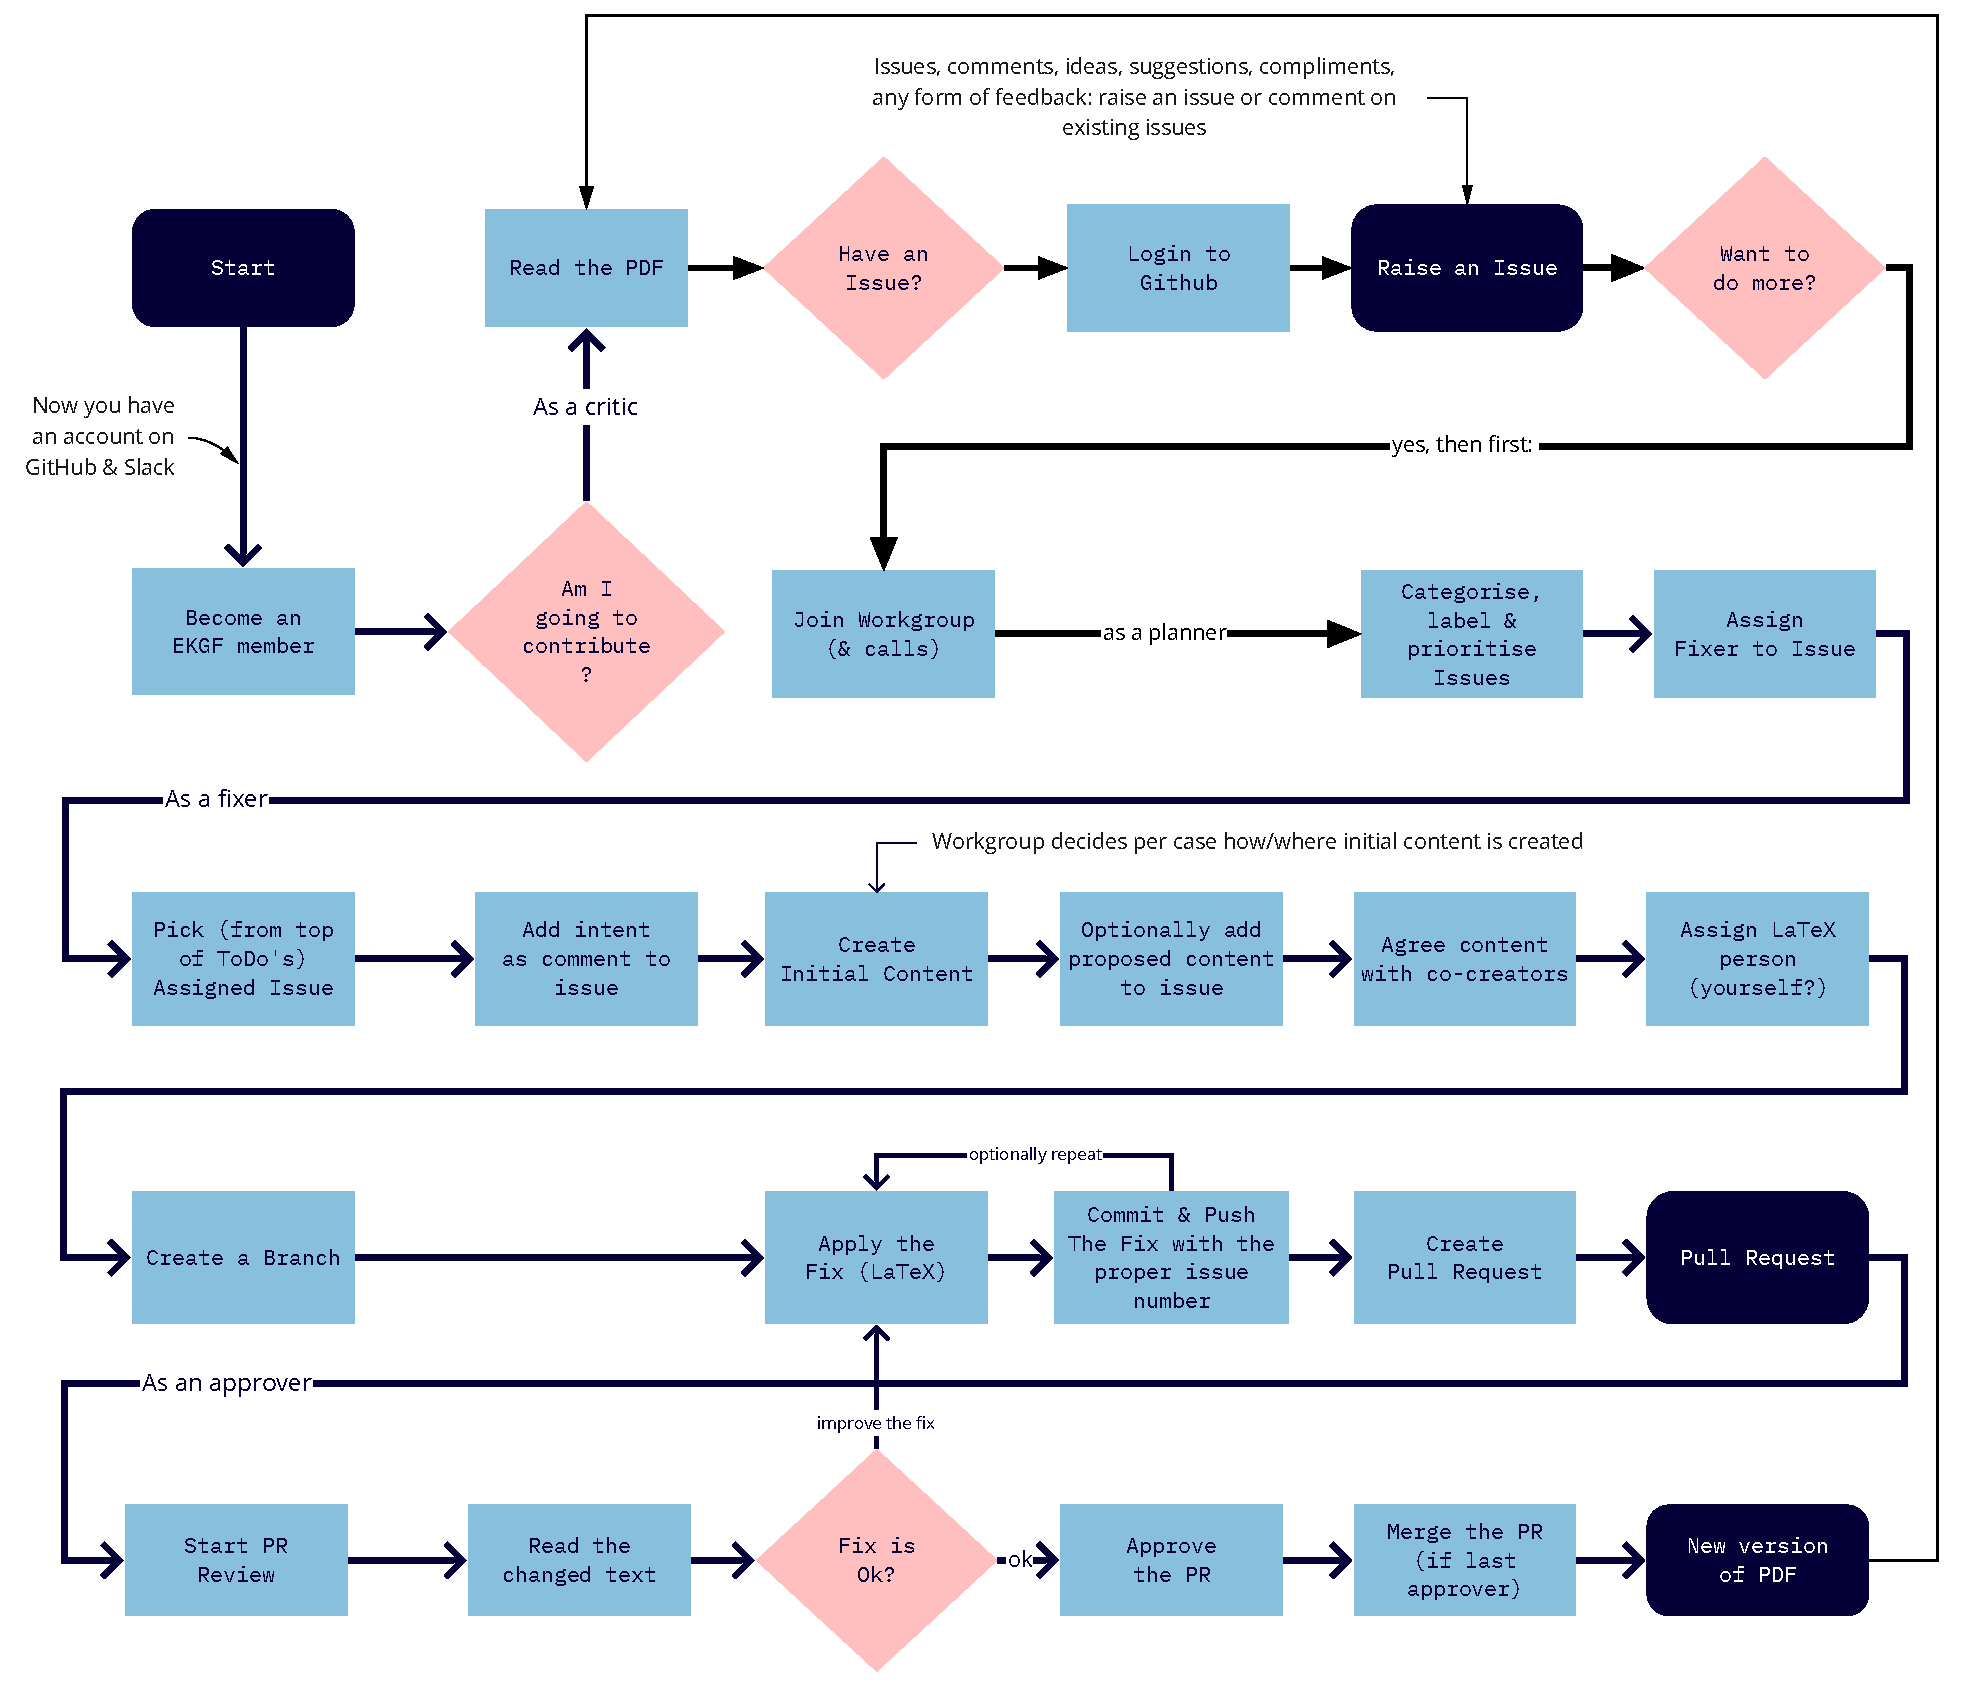
\includegraphics[width=\textwidth]{../images/ekgmm-process-diagram.pdf}
    \label{fig:ekg-mm-process-diagram}
\end{figure}

\section{Raise}
\label{sec:ekg-mm-process-raise}

\begin{tcolorbox}[colback=secondary!5,colframe=secondary!80,title=\textbf{User Stories}]
    \begin{itemize}[leftmargin=1em]
        \item As a \underline{critic}, I want to be able to \textbf{raise an issue}
    \end{itemize}
\end{tcolorbox}

Anyone who reads the produced content and has an issue with that content is a "critic".
Each critic should be able to raise that issue formally with minimal effort.

The audience of critics is hopefully very large, any reader of our content should
be able to add their comments somewhere.
We have to make it as easy as possible for them to do so. 

Unfortunately, the Issue Management function of private GitHub repositories--like
the \href{https://github.com/ekgf/ekg-mm}{EKGF/ekg-mm} repository--can only be
used by people who have a GitHub account\index{GitHub!account} (see \ref{subsec:ekg-mm-process-how-to-register}).

As someone in the role of a critic, you don’t have to deal with "\iindex{Agile}"
or "\iindex{Kanban}". 
The various workgroups/teams will plan for (see \ref{sec:ekg-mm-process-plan})
and process/fix (see \ref{sec:ekg-mm-process-fix}) your issues. 
You can always see the status of your issue by clicking on it and checking 
the right side of the screen where you see links to the "Assignee"
(the person who is going to work on your issue), the "Project"
(the workgroup that’s planning and tracking your issue) and the "Linked pull requests". 

\subsection{How to register?}
\label{subsec:ekg-mm-process-how-to-register}

We are asking every potential contributor, even someone who just wants to give us
some feedback (a "critic") to join the \gls{ekgf}.

The \gls{ekgf} supports free membership for individuals and corporate membership.

Email with \href{mailto:registration@ekgf.org}{registration@ekgf.org} to set it up,
if you plan to participate as a contributor to the \gls{ekgmm} then please also
supply your GitHub user-id\index{GitHub!account}.

\subsubsection{How to create a GitHub \& Slack account?}

\paragraph{Slack}\index{Slack}

If you already have a Slack account then join the \gls{ekgf} workspace here: \url{https://ekgf.slack.com/}.
Otherwise first create your Slack account here: \url{https://slack.com/get-started\#/create}.

\paragraph{GitHub}\index{GitHub}

Go to \url{https://github.com/join}.

Since you can associate multiple email addresses to your GitHub account we would
suggest to initially create it with your private email address which then becomes
your "primary email account" in GitHub.
You can add your business email address(es) to your GitHub account later.

Mail your GitHub account id (user-id) to
\href{mailto:registration@ekgf.org}{registration@ekgf.org} so that we can add you
to the access control list of the \href{https://github.com/EKGF/ekg-mm}{EKGF/ekg-mm repository}.

\pagebreak
\subsection{How to read the content?}

If you’re interested in the latest version of the \gls{ekgmm} document,
which is published as a PDF document, then go to
\url{https://www.ekgf.org/maturitymodel} and download it from there.

\begin{wrapfigure}[18]{r}{0.5\textwidth}
    \vspace{-12pt}
    \begin{center}
        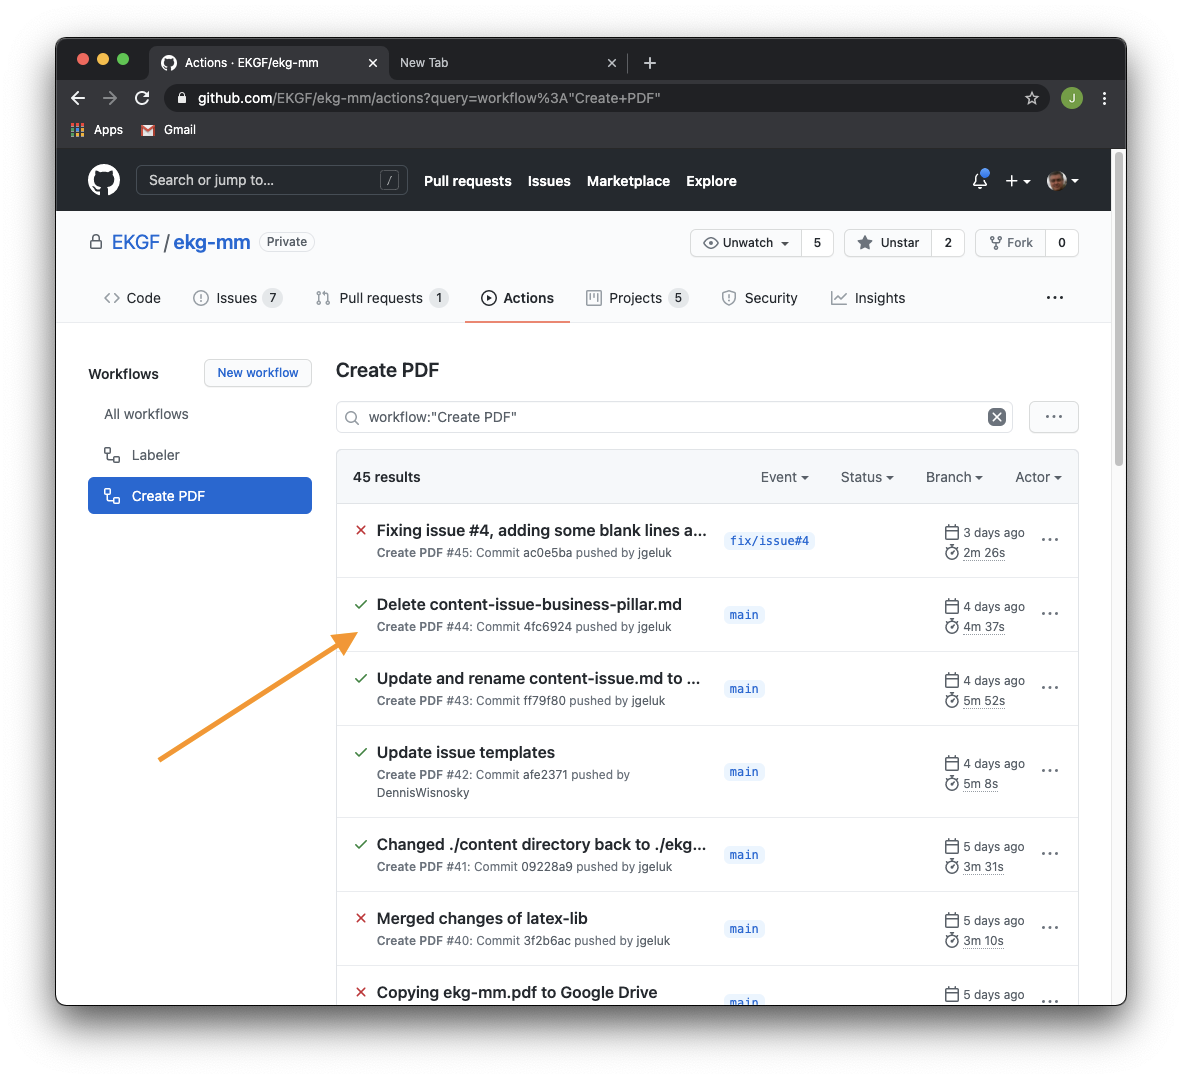
\includegraphics[width=0.50\textwidth]{../images/ekgmm-process-create-pdf-workflow.png}
    \end{center}
    \caption{Find your PDF}
    \label{fig:ekgmm-process-find-your-pdf}
\end{wrapfigure}

NOTE: At the moment we do not yet put the latest version of the generated 
PDF document on that webpage automatically so it can take a few days until 
\gls{ekgf} staff manually uploads the latest version to that webpage. 
We’re working on automating that last step of the "\gls{ci} Process".

\subsubsection{How to read specific versions of the PDF?}

For readers who would like to see “work in progress”, versions of the document 
that are being worked on in the various “branches” of the repository, 
there’s another way to get to the corresponding PDF document.

To see the latest content for any given branch, go to the "Actions" page 
on the GitHub website (\url{https://github.com/ekgf/ekg-mm/actions}) where you can 
find the \gls{ci}-build processes that create the PDF for each change 
(in git jargon that would be called "a push") in any branch.

In figure \ref{fig:ekgmm-process-find-your-pdf} you can see how you can 
find the latest successful run of the "Create PDF" workflow on the 
\texttt{main} branch (job \#44 in this case, the branch name is shown in blue).

%
% Wrap the figure on the left, give it 20 lines of vertical space and scale
% it down to half the text width
%
\begin{wrapfigure}[20]{l}{0.5\textwidth}
    \vspace{-12pt}
    \begin{center}
        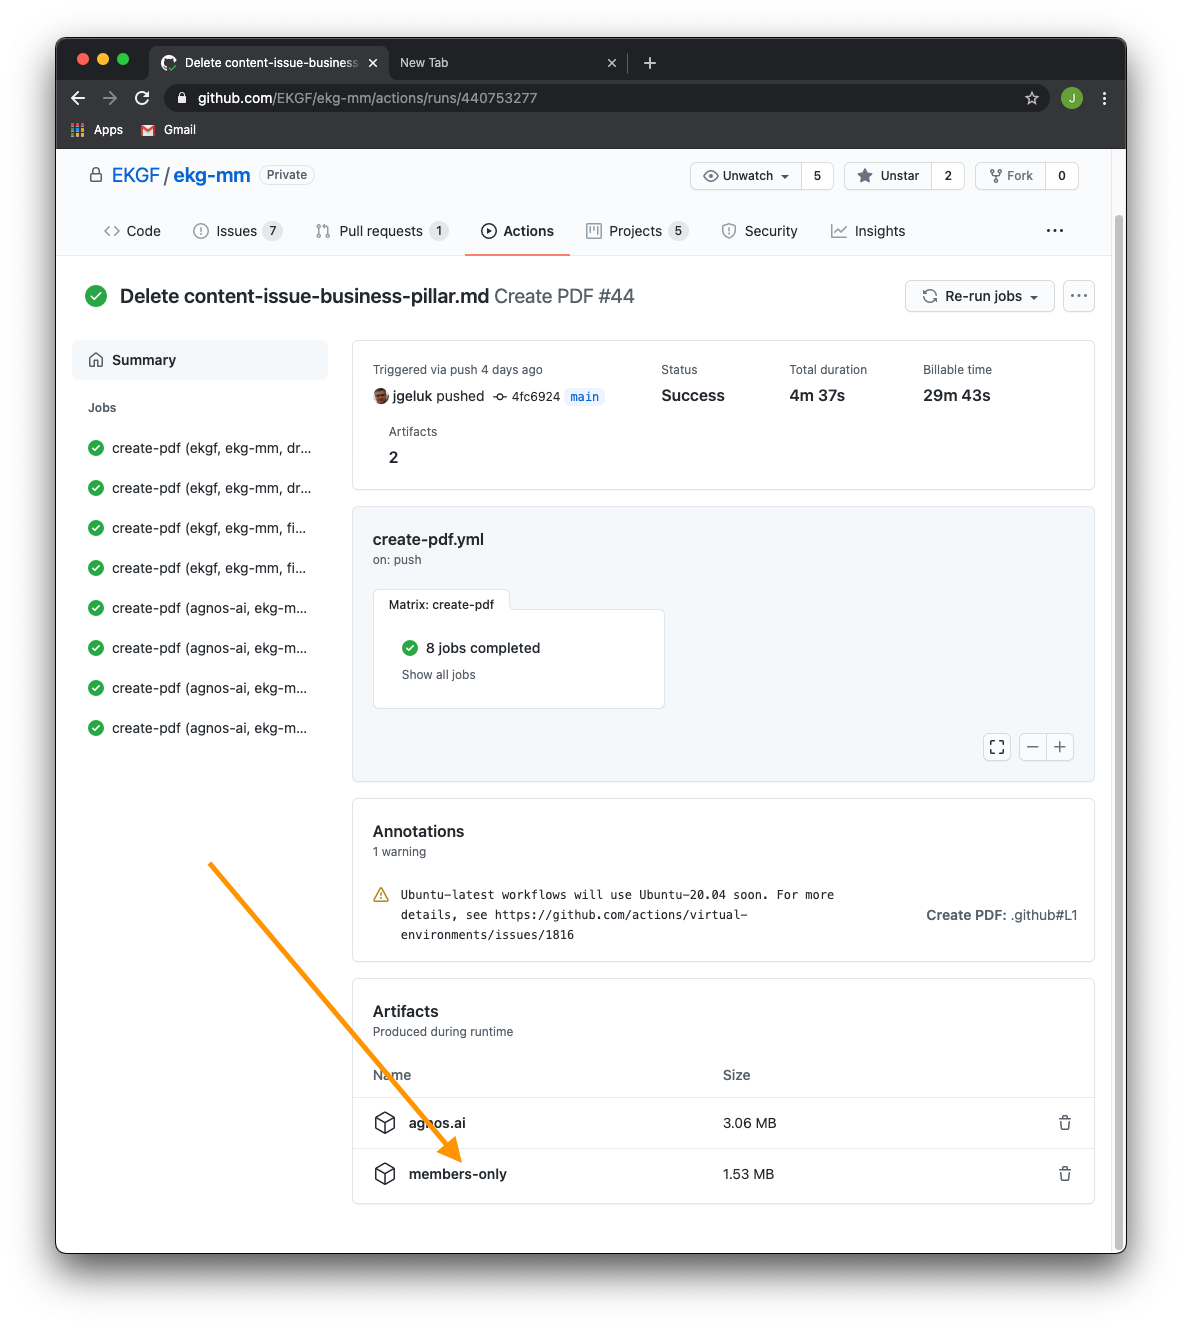
\includegraphics[width=0.50\textwidth]{../images/ekgmm-process-create-pdf-job.png}
    \end{center}
    \caption{The "Create PDF Job" page where you can find your PDF}
    \label{fig:ekgmm-process-create-pdf-job}
\end{wrapfigure}

When you then click on the name of that job, you will see the details of that job.
When the job ran successfully, "everything is green" as you can see in figure
\ref{fig:ekgmm-process-create-pdf-job}.
Scroll to the bottom where you will find the "members-only" link which gives you
a downloadable zip file with the "editors-version" and "release-version" of the document.

\subsubsection{Document File Names}
\label{subsec:ekg-mm-process-document-file-names}

The ``create-pdf'' job as shown in figures \ref{fig:ekgmm-process-find-your-pdf}
and \ref{fig:ekgmm-process-create-pdf-job} generates two different versions of the PDF:

\begin{enumerate}[leftmargin=1.2em,font=\footnotesize]
    \item {\footnotesize\texttt{ekgf-ekg-mm-<version-number>.pdf}}
    \item {\footnotesize\texttt{ekgf-ekg-mm-editors-version-<version-number>.pdf}}
\end{enumerate}

The documents with "\texttt{editors-version}" in the file name have a wider right margin
where all kinds of "notes" and "todo’s" can be shown (that are part of the content in git).
They can also contain new sections of the document that are not fully consistent yet.

\subsection{How to raise an issue?}
\label{subsec:ekg-mm-process-how-to-raise-an-issue}

While you’re reading the document, you may have comments, we hope you do.
Please raise as many "issues" as possible, any feedback is welcome.
An issue can be a question, a suggestion, a grammar issue, 
an issue with the consistency of the story, anything that comes to mind. 
If you decide to let us benefit from your feedback then please follow these steps:

\begin{itemize}
    \item Go to the main page where all issues are shown:
          \url{https://github.com/ekgf/ekg-mm/issues}
    \item Check if your issue is already raised by someone else, if so, 
          feel free to augment the discussion around that issue with your own concerns.
    \item If it clearly is a new issue, click the "New Issue" button.
    \item Give it a concise title and clear description and ideally:
    \begin{itemize}
        \item Copy paragraphs you don’t agree with into the issue
        \item Mention the paragraph number and version of the document (as shown on the front page) 
    \end{itemize}
    \item There is no need to specify values for any of the fields on
          the right side because the admin team will do that (but feel free to).
    \item Save by clicking the “Submit new issue” button
\end{itemize}

That’s it. Thank you very much. Every issue is a discussion page,
other people can respond to it and chip in. 
At some point, a workgroup will pick it up, assign it to their project board, 
plan for fixing it, etc. You will be notified of these changes 
automatically via GitHub email.

\section{Plan}
\label{sec:ekg-mm-process-plan}

\begin{tcolorbox}[colback=secondary!5,colframe=secondary!80,title=\textbf{User Stories}]
    \begin{itemize}[leftmargin=1em]
        \item As a \underline{planner}, I want to be able to \textbf{plan issues}
    \end{itemize}
\end{tcolorbox}

Work on the \gls{ekgmm} is divided among workgroups that each take on an MM pillar
or horizontal slice of the MM. 
Workgroups are self-managed teams. 
The workgroups meet on a regular schedule. 
Any method that the team agrees to use to plan and to document issues during 
working sessions is ok. 
But, the official content of the MM is contained in the GitHub repository 
that is managed using the GitHub Kanban with review and automation process.

Here are some useful links. 

\begin{itemize}
    \item \href{https://www.atlassian.com/agile/kanban}{Kanban - A brief introduction}
    \item \href{https://www.atlassian.com/agile/kanban/boards}{What is a Kanban Board?}
\end{itemize}

The idea is very simple though, we use the GitHub Projects facility. 
Currently, we have a project for each pillar and a general project. 
Here’s the main page for \gls{ekgmm} GitHub Projects:

\begin{center}
    \url{https://github.com/ekgf/ekg-mm/projects}
\end{center}

What you see is a list of "project boards" where each project board 
is owned by a workgroup in the entire Kanban process. 
This begins with planning. 

The planning process consists of various tasks:

\begin{itemize}
    \item Find open issues that are relevant to the workgroup in the list of issues:
    \begin{itemize}
        \item Here is a link: \href{https://github.com/EKGF/ekg-mm/issues?q=is%3Aissue+is%3Aopen+no%3Aproject}
              {open issues that have not yet been assigned to a project board}
    \end{itemize}
    \item Link each issue that should be done by the workgroup to its
          corresponding project board.
          It will then appear at the bottom of the “To Do” column of that board.
    \item Decide priority (see \ref{subsec:ekg-mm-process-to-do-column}).
    \item Assign issues to members of the workgroup.
    \begin{itemize}
        \item By linking the issue to one or more assignees
              (open the issue by clicking on it and select the assignee at
              the top right corner)
    \end{itemize}
    \item Follow the progress of issues as they go from left to right via the columns on the board.
\end{itemize}

\subsection{"To Do" Column}
\label{subsec:ekg-mm-process-to-do-column}

As soon as an issue has been assigned to a given project, 
it will show up at the bottom of the To-Do Column\index{GitHub!Issue Management}.
That To-Do Column can be seen as "the \iindex{backlog}"
for that project (and for the workgroup that owns that project).

Issues can be dragged and dropped within the To-Do Column. 
Issues at the top have the highest priority. 
Anyone in the workgroup can pick up issues assigned to 
them and start "fixing" them (which means resolving them), 
see \secref{sec:ekg-mm-process-fix}.

\subsection{"In progress" Column}\index{GitHub!Issue Management}

Pull Requests and Issues\footnote{Issues are sometimes also 
called “Cards” in Kanban terminology and in the Github project 
user interface.
Besides that you can also add “Notes” to the project board.} 
show up in this column automatically as soon as someone is 
actually working on the issue, see \secref{sec:ekg-mm-process-fix}.

This means that as soon as a fixer "pushes" one or more "commits" 
to the GitHub repository that this will be seen as progress 
and show up accordingly on the project board.

\subsection{"Review in progress" Column}\index{GitHub!Issue Management}

Once the fixer has created their \gls{pr}, they can ask 
for a review of the \gls{pr} by selecting two or more reviewers. 
See \secref{sec:ekg-mm-process-approve} for information about how to do a review.

\subsection{"Reviewer approved" Column}\index{GitHub!Issue Management}

Once all reviewers have approved the \gls{pr}, 
the last reviewer can then merge the \gls{pr} into the main branch. 
By the way, a reviewer can also reject a change or ask for 
changes to be applied before approving the \gls{pr}. 

The fixer then has to then apply new changes and commit 
them to the same branch and push those changes to GitHub. 
The \gls{pr} page will then be updated automatically and a subsequent 
review process can then commence.
As said above, once all approvals are given, 
the changes can then be merged by the final reviewer 
into the main branch which will trigger the final build 
workflow on GitHub creating the publishable content as 
PDF (and eventually also as HTML).

\subsection{"Done" Column}\label{subsec:ekg-mm-process-done-column}
\index{GitHub!Issue Management}

When the merge of the \gls{pr} is done the issue will move to 
the Done column. 

For each \gls{pr} there is an underlying git branch which 
will be automatically deleted by GitHub once the \gls{pr} 
has been merged into the main branch.

\pagebreak
\section{Fix}
\label{sec:ekg-mm-process-fix}

\begin{tcolorbox}[colback=secondary!5,colframe=secondary!80,title=\textbf{User Stories}]
    \begin{itemize}[leftmargin=1em]
        \item As a \underline{fixer}, I want to be able to \textbf{fix issues}
        \item As a \underline{fixer}, I want to be able to \textbf{create a pull request}
    \end{itemize}
\end{tcolorbox}

The term "\iindex{fixer}" is our own term, they’re usually called "developer" but
we don’t consider someone who works on \gls{ekgmm} content to be a developer necessarily.
In the GitHub user interface, they show up as "contributors"\index{contributor}.
Anyone who actually changes things in the repository will be registered by GitHub as 
a contributor to that repository\footnote{The GitHub userids and names of all 
contributors will be listed in the final output \gls{ekgmm} document.}.

There are many different ways to change the content of the repository. 
There are roughly two methods though:

\begin{enumerate}[label=(\Alph*)]
    \item Change content without making a "clone" of the repository by editing content on the GitHub site itself.
    \item Make a so-called "git clone" of the repository to your own workstation and use any appropriate editor to add or change things.
\end{enumerate}

%
% Wrap the figure on the left, give it 20 lines of vertical space and scale
% it down to half the text width
%
\begin{wrapfigure}[16]{r}{0.5\textwidth}
    \vspace{-12pt}
    \begin{center}
        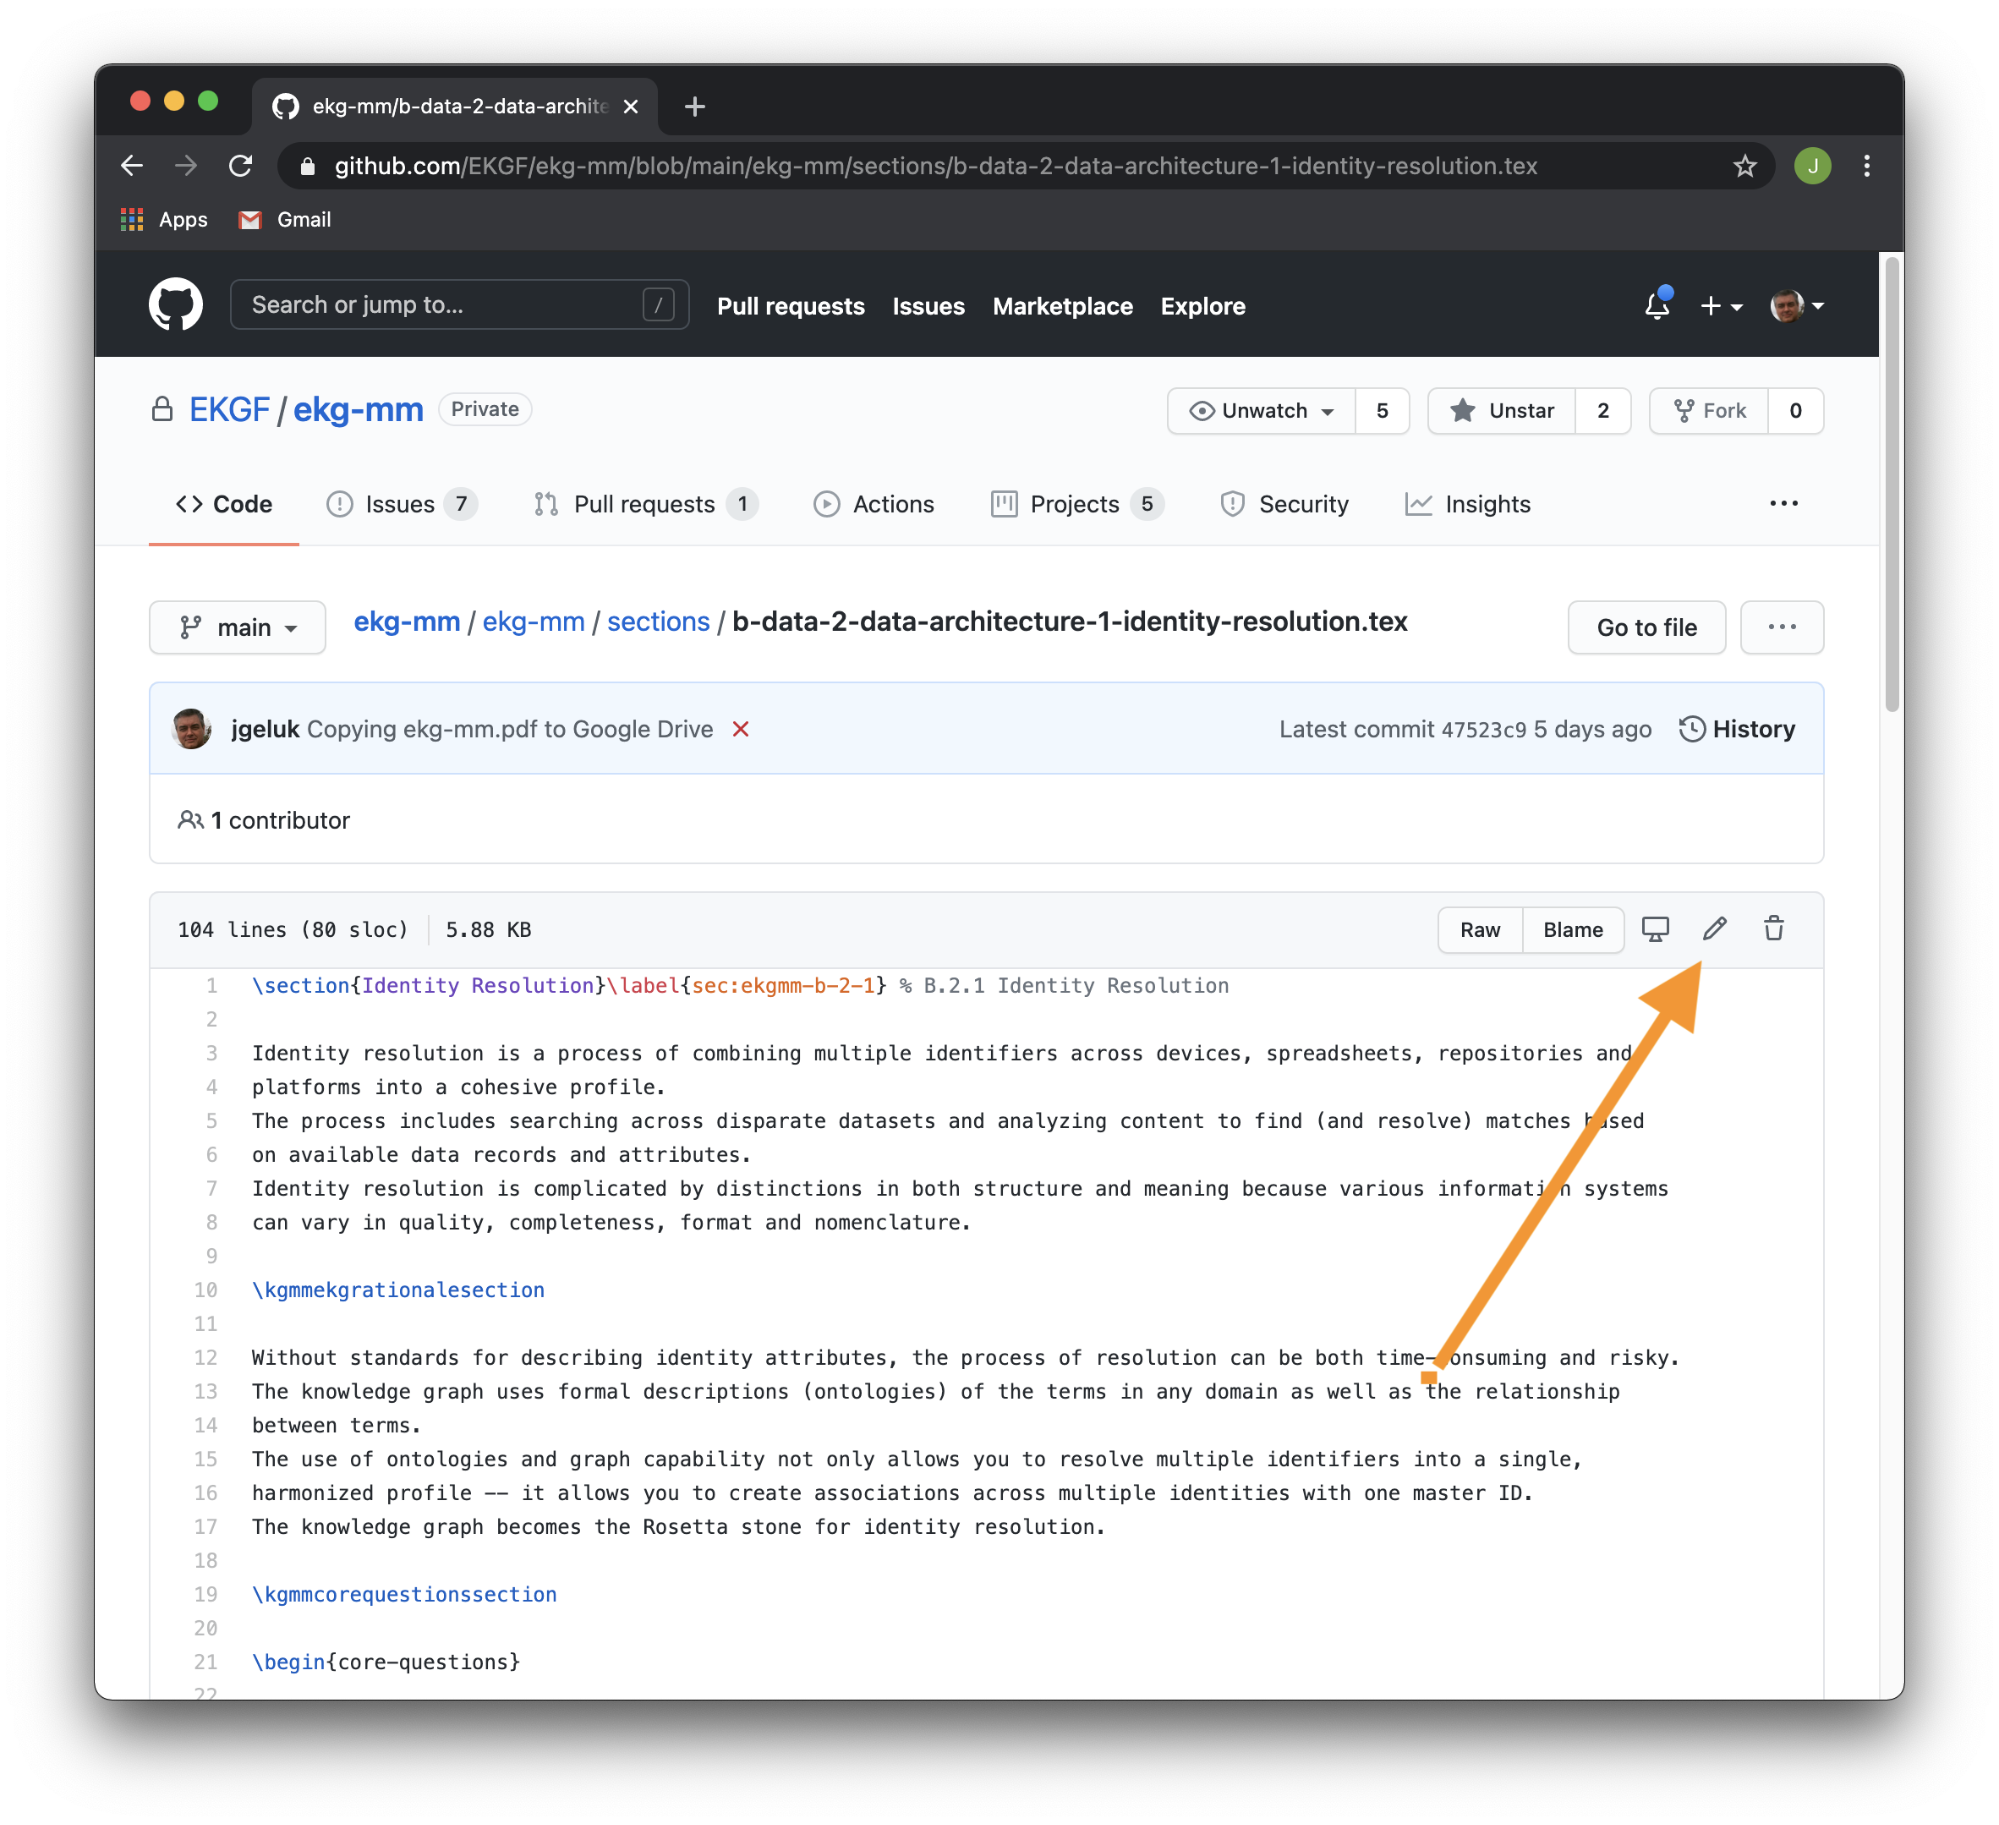
\includegraphics[width=0.50\textwidth]{../images/ekgmm-process-edit-content.png}
    \end{center}
    \caption{Where to find the edit button}
    \label{fig:ekgmm-process-edit-content}
\end{wrapfigure}

Both methods require:

\begin{itemize}
    \item "creating a branch" (See \ref{subsec:ekg-mm-process-how-to-make-a-branch})
    \item "committing a change" (See \ref{subsec:ekg-mm-process-how-to-commit})
    \item "creating a pull request" (See \ref{subsec:ekg-mm-process-how-to-create-a-pull-request})
\end{itemize}

We will now describe how each of these three tasks can be done.

\subsection{How to start editing in GitHub?}

This is "Method A" as described above.
First find the content file that you want to edit.
All content is under the content root directory \texttt{/ekg-mm}.

The arrow in figure \ref{fig:ekgmm-process-edit-content} above shows the
location of the "edit button" (ignore the other buttons). 
Click that button and change any content. 
All content is written in a "language" called \iindex{LaTeX} which is
a markup language for professional content (used for books and Ph.D. 
thesis and the like).
As long as you keep the LaTeX commands (aka macros) in place (they 
start with a backslash) things will be fine, just type away. 
Unless you know LaTeX (a little) then you can add whatever works.

Then it’s time to save the changes, choose a good title for your 
change, and include the issue number (for instance \texttt{\#123})
prefixed with a hash.
This title is the so-called "commit message" and is described in 
more detail in \subsecref{subsec:ekg-mm-process-how-to-commit}.

\subsection{How to make a branch?}
\label{subsec:ekg-mm-process-how-to-make-a-branch}

When editing straight on the GitHub site as described in the previous 
section, you have to save your work "as a commit" with a title that 
contains the issue number (which will be picked up by the project board). 
But you then also have to create a branch which shows up right under 
the title and description. 

Choose a branch name that explains what it is about. 
In some cases that would be all there is to it but in most cases you 
have multiple edits in multiple files for one given issue. 
So in those cases you would have to make sure to always refer to 
the right branch name where the branch name must include the 
issue number itself. 
For instance, for issue \texttt{\#123} the branch name would 
be \texttt{issue-123}.

\subsection{How to commit a change?}
\label{subsec:ekg-mm-process-how-to-commit}

%
% Wrap the figure on the left, give it 20 lines of vertical space and scale
% it down to half the text width
%
\begin{wrapfigure}[20]{l}{0.5\textwidth}
    \vspace{-12pt}
    \begin{center}
        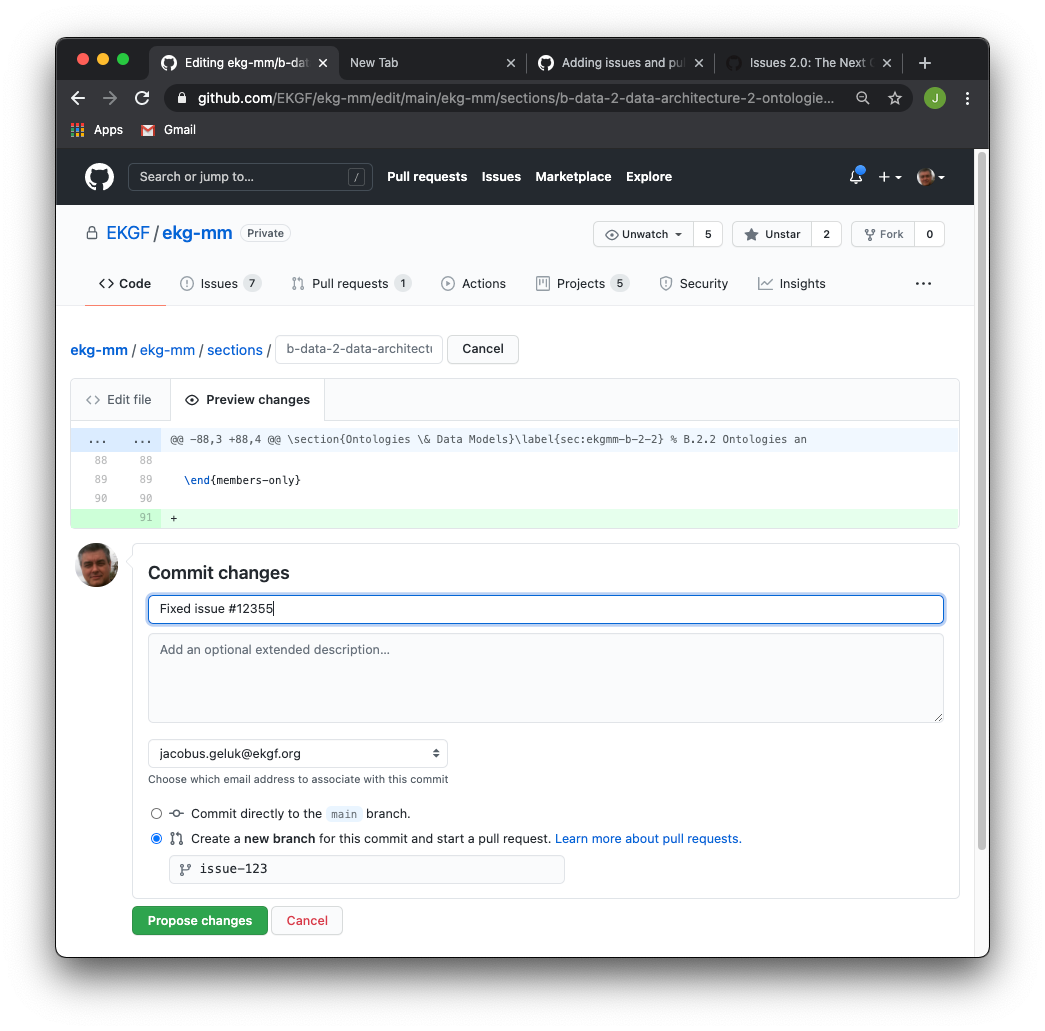
\includegraphics[width=0.50\textwidth]{../images/ekgmm-process-commit-changes.png}
    \end{center}
    \caption{Committing changes}
    \label{fig:ekgmm-process-commit-changes}
\end{wrapfigure}

There are many different ways to create a commit on a branch in a 
git repository. It’s up to the "fixer" (usually called "developer"
in most git documentation on the Internet) to decide which
tooling they use.
One way to do this is to just use the Github website itself but you
could also create a so-called "clone" of the git repository on your 
local machine and use the standard git utility to create a commit or 
use an advanced editor like Visual Studio Code that has built-in 
git support and a LaTeX plugin. 
It goes too far to document all the various different ways to do this 
in the context of this document.
What’s important to know is that, as a fixer, you should always include
the issue number in the title of the commit. 
For example, if you edit a content page and then commit that change, 
you have to make sure that these two things are done before clicking 
the "Propose Changes" button as shown in figure \ref{fig:ekgmm-process-commit-changes}.

Use a title for your commit that includes the issue number, 
prefixed by \texttt{\#}, for example, \texttt{\#123} for issue 123.
Use a branch name that includes the issue number (no hash as a prefix).

The \texttt{\#123} in the title will trigger GitHub to move the
corresponding issue from the "To Do" column to the "In Progress" column.
Do not use "Fixed \texttt{\#123}" or “Close \texttt{\#123}” because that 
will actually close the issue.

Once you have done your first commit to a given branch, you’re ready to
create a \gls{pr}. 
Many people wait with creating a \gls{pr} until their last commit is pushed
(one issue can involve many commits involving many files but they all 
go to the same branch) but we recommend creating your \gls{pr} as soon as possible, 
after the first commit, because that gives everyone an easier insight 
in the progress. Not everyone is up for that, “exposing” their 
first draft changes to others, but it’s generally seen as 
good practice to do so. 
You can mark your \gls{pr} as “Draft” via the GitHub user interface so that 
everyone knows that it is “work in progress”.

\subsection{How to create a pull request?}
\label{subsec:ekg-mm-process-how-to-create-a-pull-request}

Assuming that you added some changes to a branch, in GitHub parlance: 
"pushed some commits to a branch", you can also create a \gls{pr}. 
A \gls{pr} can be seen as a "request approval to change"-form. 
It needs two branches: the branch that you want to change (that would 
usually be the main branch) and the branch that contains the new version 
with the proposed changes. 
GitHub automatically calculates the difference between those two branches
and shows those differences on the \gls{pr}-form.

There are several different places in the GitHub user interface where you 
can start creating a \gls{pr} but the most basic one shows up at the branches 
page which shows all branches of the repository:

\begin{center}
    \url{https://github.com/ekgf/ekg-mm/branches}
\end{center}

On the right side of the table showing all the branches you either see an 
existing \gls{pr} for the given branch or a button:

\begin{center}
    
\includegraphics[scale=0.5]{../images/ekgmm-process-pr-button.png}
\end{center}

It’s easy from there. 
Give your \gls{pr} a good title (that title goes into the "changelog" so be 
specific) and a description and click the Create Pull Request button. 
Job done. A planner in the workgroup will take it from there, 
assign reviewers, link it to a project board etc.

\section{Approve}
\label{sec:ekg-mm-process-approve}

\begin{tcolorbox}[colback=secondary!5,colframe=secondary!80,title=\textbf{User Stories}]
    \begin{itemize}[leftmargin=1em]
        \item As a \underline{reviewer}, I want to be able to \textbf{approve pull requests}
    \end{itemize}
\end{tcolorbox}

TODO


\typeout{ekg-mm =================================> Appendix: History}
\chapter{History}

\begin{version-history}
    0.1 & 01/03/2019 & \agnos started with the \glsfmtshort{ekgmm} initiative & Michael Atkin, Jacobus Geluk \\
    0.1 & 01/01/2020 & \agnos donated IP to \glsfmtshort{ekgmm} to EKGF ``as is'' & Jacobus Geluk \\
    0.2 & 01/01/2021 & Started with new delivery process & Mike Atkin, Dennis Wisnosky \\
    0.3 & 08/04/2021 & Business pillar workgroup deciding top-level structure & Lars Magnusson, Carl Mattocks, Jeffrey Wallk \textit{et al}. \\
    0.4 & 27/05/2021 & New intro for business pillar & Avinash Patil, Carl Mattocks, \textit{et al} \\
        &            & Content for \ref{sec:ekg-mm-change-management} \nameref{sec:ekg-mm-change-management} & Diane Alexander, Jeffrey Wallk \\
        &            & Removed chapter "A.1.4 Operating Model" &  \\
        &            & Added content for chapter "A.3.3 Risk Management" & Diane Alexander \\
    0.5 & 08/06/2021 & Added appendix "What is Strategy?" & Carlos Tubbax \\
        &            & Added several updates to Business Pillar intro &  Avinash Patil \\
    0.6 & 14/06/2021 & Added chapter "A.3.1 Operating Model" & Carlos Tubbax \\
    0.7 & 01/07/2021 & Moved operating model version of Carlos to Appendix and added a new appendix "Enterprise Architecture" & Carlos Tubbax \\
    0.8 & 31/08/2021 & Added completely new content for "B.2.2 Ontologies" & Pete Rivett and others \\
        &            & Added completely new content for "A.3.2 Enterprise Architecture" & Carlos Tubbax \\
        &            & A.3.2 Performance Management is now A.3.3 Performance Management &  \\
        &            & A.3.3 Risk Management is now A.3.4 Risk Management &  \\
        &            & A.3.4 Supply Chain Management is now A.3.5 Supply Chain Management &  \\
        &            & Removed A.3.2 Enterprise Architecture, moved it to appendix & \\
    0.9 & 05/10/2021 & Reshuffle of various capabilities in Data Pillar & Pete Rivett \\
   0.10 & 13/10/2021 & Moved Organization Pillar to second place & Avinash Patil \\
   0.11 & 26/10/2021 & Added chapter A.3.5 Capability Map & Carlos Tubbax \\
\end{version-history}


\typeout{ekg-mm =================================> Appendix: Contributors}
\chapter{Contributors}

All contributors in alphabetical order.

TODO: Many people have not been added yet!! Work in progress!!

\begin{table}[ht]
    \small
    \let\freewidth\relax%
    \newlength{\freewidth}%
    \setlength{\freewidth}{\dimexpr\textwidth-8\tabcolsep}%
    \renewcommand{\arraystretch}{1.5}%
    \begin{tabular}{
        @{}
        p{0.30\freewidth}
        p{0.30\freewidth}
        p{0.30\freewidth}
        @{}
    }
        \textbf{Contributor} & \textbf{Org} & \textbf{Role} \\ \toprule
        \href{https://www.linkedin.com/in/diane-alexander-pmp-ssbb/}{Diane Alexander} & \href{https://factorfirm.com/}{Factor} & Business Pillar \\
        \href{https://www.linkedin.com/in/matkin/}{Michael Atkin} & Columbia University & EKGF Founder \newline EKG/MM Initiator \newline Data Pillar \\
        \href{https://www.linkedin.com/in/jgeluk/}{Jacobus Geluk} & \agnos & EKGF Founder \newline EKG/MM Initiator \newline Business/Data/Tech pillars \\
        \href{https://www.linkedin.com/in/howard-knowles-57815b6/}{Howard Knowles} & \agnos & Technology Pillar \\
        \href{https://www.linkedin.com/in/ross-leher-4471971/}{Ross Leher} & \href{https://www.wandinc.com}{WAND} & Business Pillar \\
        \href{https://www.linkedin.com/in/marylevins/}{Mary Levins} & \href{http://www.sierracreekconsulting.com/}{Sierra Creek Consulting} & Business \& Data Pillar \\
        \href{https://www.linkedin.com/in/larsmmagnusson/}{Lars Magnusson} & Ericsson & Business Pillar \\
        \href{https://www.linkedin.com/in/carlmattocks/}{Carl Mattocks} & GE & Business Pillar \\
        \href{https://www.linkedin.com/in/jeduardomtz/}{Eduardo Martinez} & BMO & Business Pillar \\
        \href{https://www.linkedin.com/in/avinash-patil-4229564/}{Avinash Patil} & Tata Consultancy Services & Business Pillar \\
        \href{https://www.linkedin.com/in/peterivett/}{Pete Rivett} & OMG \newline \agnos & EKGF Founder \& Vice President \newline Data Pillar \\
        \href{https://www.linkedin.com/in/msls07/}{Marina Severinovskaya} & Citi & Business \& Data Pillar \\
        \href{https://www.linkedin.com/in/carlos-tubbax-975058118/}{Carlos Tubbax} & \href{https://www.uantwerpen.be/en/staff/carlos-tubbax/}{University of Antwerp} & Business Pillar \\
        \href{https://www.linkedin.com/in/jeffreywallk/}{Jeffrey Wallk} & \href{https://www.enablingvalue.com}{Value Enablement Group} & Business Pillar \\
        \href{https://www.linkedin.com/in/denniswisnosky/}{Dennis Wisnosky} & Wizdom & EKGF Founder \& Chair \newline EKG/MM Process \\
        \href{https://www.linkedin.com/in/jeanninewisnoskystehlin/}{Jeannine~Wisnosky Stehlin} & Wizdom & EKGF Director of operations \newline EKG/MM Process \\
        \bottomrule
    \end{tabular}
\end{table}


\typeout{ekg-mm =================================> Appendix: Corporate Members}
\chapter{Corporate Members}
\label{appendix:ekgf-corporate-members}

The corporate members of the \glsfirst{ekgf} currently are\,---\,ordered by join date:

\paragraph{\agnos}
\label{agnos}
\index{agnos.ai}

\href{https://agnos.ai}{agnos.ai} is an Enterprise Knowledge Graph consultancy assisting its clients in
their \gls{ekg} journey from strategy to production.

\paragraph{Wizdom}
\label{wizdom}
\index{wizdom}

\href{http://www.wizdom.com/}{Wizdom} is a recognized leader in providing our clients with
innovative process-based business solutions for improving performance.

\paragraph{\stardogcompany}
\label{stardog}
\index{stardog}
\index{stardog!\glsfmtshort{ekg} platform}

\href{https://www.stardog.com/}{Stardog}, the leading Enterprise Knowledge Graph platform,
turns data into knowledge to power more effective digital transformations.

\paragraph{\ontotext}
\label{ontotext}
\index{ontotext}
\index{ontotext!GraphDB}

\href{https://www.ontotext.com/}{Ontotext} is a global leader in enterprise knowledge graph technology
and semantic database engines.

\paragraph{\dataworld}
\label{dataworld}
\index{data.world}

\href{https://data.world}{data.world} makes it easy for everyone—not just the "data people"—to get clear, accurate,
fast answers to any business question.

\paragraph{\eccenca}
\label{eccenca}
\index{eccenca}
\index{eccenca!corporate memory}

\href{https://eccenca.com/}{eccenca} is a leading provider of enterprise knowledge graph management
software and solutions.

\paragraph{Global IDs}
\label{globalids}
\index{global ids}

\href{https://www.globalids.com/}{Global IDs} provides software for enterprise information management (EIM).

\paragraph{\cambridgesemantics}
\label{cambridgesemantics}
\index{cambridge semantics}
\index{cambridge semantics!anzo}

\href{https://www.cambridgesemantics.com/}{Cambridge Semantics} provides Anzo,
the scalable knowledge graph platform for data integration and analytics.







\end{document}
